\documentclass{book}
\usepackage[a4paper,top=2.5cm,bottom=2.5cm,left=2.5cm,right=2.5cm]{geometry}
\usepackage{makeidx}
\usepackage{natbib}
\usepackage{graphicx}
\usepackage{multicol}
\usepackage{float}
\usepackage{listings}
\usepackage{color}
\usepackage{ifthen}
\usepackage[table]{xcolor}
\usepackage{textcomp}
\usepackage{alltt}
\usepackage{ifpdf}
\ifpdf
\usepackage[pdftex,
            pagebackref=true,
            colorlinks=true,
            linkcolor=blue,
            unicode
           ]{hyperref}
\else
\usepackage[ps2pdf,
            pagebackref=true,
            colorlinks=true,
            linkcolor=blue,
            unicode
           ]{hyperref}
\usepackage{pspicture}
\fi
\usepackage[utf8]{inputenc}
\usepackage[french]{babel}

\usepackage{mathptmx}
\usepackage[scaled=.90]{helvet}
\usepackage{courier}
\usepackage{sectsty}
\usepackage{amssymb}
\usepackage[titles]{tocloft}
\usepackage{doxygen}
\lstset{language=C++,inputencoding=utf8,basicstyle=\footnotesize,breaklines=true,breakatwhitespace=true,tabsize=8,numbers=left }
\makeindex
\setcounter{tocdepth}{3}
\renewcommand{\footrulewidth}{0.4pt}
\renewcommand{\familydefault}{\sfdefault}
\hfuzz=15pt
\setlength{\emergencystretch}{15pt}
\hbadness=750
\tolerance=750
\begin{document}
\hypersetup{pageanchor=false,citecolor=blue}
\begin{titlepage}
\vspace*{7cm}
\begin{center}
{\Large I\-G\-Osat Simulator }\\
\vspace*{1cm}
{\large Généré par Doxygen 1.8.1.2}\\
\vspace*{0.5cm}
{\small Samedi Mai 10 2014 18:35:55}\\
\end{center}
\end{titlepage}
\clearemptydoublepage
\pagenumbering{roman}
\tableofcontents
\clearemptydoublepage
\pagenumbering{arabic}
\hypersetup{pageanchor=true,citecolor=blue}
\chapter{Simulateur I\-G\-O\-Sat}
\label{index}\hypertarget{index}{}\hypertarget{index_intro_sec}{}\section{Introduction}\label{index_intro_sec}
Dévelloppé dans le cadre d'un projet de master, ce programme pose les bases d'un simulateur de système complexe écrit en C++, basé sur des modules abstraits synchronisés via une horloge.\hypertarget{index_general}{}\section{Principe général de la simulation}\label{index_general}
L'idée du simulateur est de représenter le satellite comme un ensemble de modules ordonnés hiérarchiquement. Trois briques de base sont disponible\-: les \hyperlink{docModule}{modules}, les \hyperlink{docMacroModule}{macromodules} et les modules physique. Les modules sont des éléments finaux, qui n'en contiennent pas d'autres. Les macromodules sont des modules qui peuvent contenir d'autres modules et des connexions entre ces modules. Enfin les modules physiques sont un peu à part, il serviront à modéliser, et à synchroniser avec les modules du satellite, les différents phénomènes physiques impliqués dans la simulation.

Des modules connectés au sein d'un macromodules peuvent communiquer entre-\/eux en s'envoyant des messages. Il est nécessaire de définir pour chaque module la liste des messages qu'ils est capable de comprendre ainsi que les traitements associés à la réception de chacun de ces messages.

Tous ces modules agissent de façon synchrone. Une classe \hyperlink{classTimer}{Timer} se charge d'appeller la méthode \hyperlink{classModule_ab7ea9648fa500696c85e93ebd0666390}{Module\-::clock} de chaque module à chaque pas de temps. Tous les modules sont automatiquement inscris dans le timer lors de leur construction. Il est également possible de désynchroniser certains modules, afin qu'ils tournent à une fréquence plus ou moins élevée.

Les modules peuvent êtres en partie configurés via les \hyperlink{xmlRef}{fichiers xml} qui leur sont associés, cependant cette foncitonnalité n'est pas encore complète, et le générateur associé ne peut pour le moment éditer un X\-M\-L déjà créé.\hypertarget{index_struc}{}\section{Structure du dépôt}\label{index_struc}
\begin{DoxyVerb}IGOgen/                        Générateur de code
IGOsim/                        Simulateur
   | config/                   Fichiers de configuration XML
   | doc/                      Documentation générée par Doxygen
   | src/                      Sources du simulateur
       | Core/                 Sources génériques du simulateur
       | Satellite/            Sources spécifiques à IGOsat
   | doxy.conf                 Fichier de configuration de Doxygen
ProjetM1/                      Divers pour suivi du projet
UML/                           Modélisation du simulateur
README.md                      Readme basique, affiché sur accueil du dépôt
CHANGELOG.md                   Changelog
\end{DoxyVerb}
\hypertarget{index_install_sec}{}\section{Installation}\label{index_install_sec}
\hypertarget{index_tools_subsec}{}\subsection{Récupération des sources}\label{index_tools_subsec}
La méthode la plus simple pour récupérer les sources du projet est de cloner le dépôt depuis Git\-Hub\-: \begin{DoxyVerb}git clone https://github.com/VooDooS/Projet_Simulateur_IGOSAT.git
\end{DoxyVerb}
\hypertarget{index_tools_cofig}{}\subsection{Configuration}\label{index_tools_cofig}
Par défaut, le simulateur va aller chercher des fichiers de configuration dans le dossier {\itshape config/}, si ce n'est pas votre cas, pensez à modifier la ligne correspondante dans I\-G\-O\-Sim.\-cpp, avant de compiler. Un / doit impérativement conclure le lien. \begin{DoxyVerb}XMLReader::setPath("Path/to/config/");
\end{DoxyVerb}
\hypertarget{index_tools_compil}{}\subsection{Compilation des sources}\label{index_tools_compil}
Un makefile est fourni, pour compiler, placez vous dans le dossier src, et écecutez la commande Make\-: \begin{DoxyVerb} cd IGOSim/src/
 make
\end{DoxyVerb}
\hypertarget{index_particip}{}\section{Comment participer ?}\label{index_particip}
Si vous n'êtes pas un collaborateur du projet sur Github il vous faut créer une bifurcation (un fork) du dépôt sur votre propre compte. Il vous est ensuite possible de nous proposer vos modifications via une demande d'ajout (pull request).

Sinon, pensez à créer une branche pour effectuer vos modifications en toute sécurité, et de demander une vérification commune via une demande d'ajout. Ce processus à l'avantage de permettre à tous d'être tenus au courant de l'évolution du code.

Il est de plus fortement conseillé de tenir à jour le document \char`\"{}\-C\-H\-A\-N\-G\-E\-L\-O\-G.\-md\char`\"{}, notamment lorsque les modifications concernent la partie Core du code. 
\chapter{Référence Création Macro-\/\-Module}
\label{docMacroModule}
\hypertarget{docMacroModule}{}
\hypertarget{docModule_classCreation}{}\section{Création d'une nouvelle classe}\label{docModule_classCreation}
Pour créer un nouveau macro-\/module, il faut hériter une nouvelle classe de la classe \hyperlink{classMacroModule}{Macro\-Module}. {\itshape Remarque\-: la classe \hyperlink{classMacroModule}{Macro\-Module} est héritée de \hyperlink{classModule}{Module}, un macro-\/module est donc un module.}

Par exemple pour créer le macro-\/module {\bfseries \hyperlink{classBatteryModule}{Battery\-Module}}\-: {\ttfamily class \hyperlink{classBatteryModule}{Battery\-Module}\-:public \hyperlink{classMacroModule}{Macro\-Module}\{\};}

Il faut également au moins redéfinir deux methodes\-:
\begin{DoxyEnumerate}
\item le constructeur Macro\-Module\-::\-Macro\-Module
\item Macro\-Module\-::process (qui est héritée de Module\-::process)
\end{DoxyEnumerate}

Notez que le constructeur de votre nouveau module doit appeller le constructeur de base de la classe \hyperlink{classMacroModule}{Macro\-Module}\-:


\begin{DoxyCode}
\hyperlink{classBatteryModule_a2fb494ef5f124c38c0fdf9ccfb31918f}{BatteryModule::BatteryModule}(std::string name, 
      Params params) : \hyperlink{classMacroModule}{MacroModule}(name, params, \textcolor{stringliteral}{"
      BatteryModule/BatteryModule.xml"})\{
    \textcolor{comment}{/* ce qu'il faut faire pendant la création d'un module */}
\}
\end{DoxyCode}


Les arguments de ce constructeur de base sont les suivants\-:
\begin{DoxyEnumerate}
\item name \-: le nom de votre macro-\/module.
\item params \-: un objet de type {\ttfamily std\-::unordered\-\_\-map$<$std\-::string, double$>$} avec des paramètres d'un macro-\/module.
\item \char`\"{}\-Battery\-Module/\-Battery\-Module.\-xml\char`\"{} – le chemin vers le fichier {\ttfamily .xml} qui contient la configuration du module.
\end{DoxyEnumerate}\hypertarget{docModule_properties}{}\section{Propriétés d'un Module}\label{docModule_properties}
\hypertarget{docMacroModule_submodules}{}\subsection{Sous-\/modules}\label{docMacroModule_submodules}
La difference principale entre \hyperlink{classModule}{Module} et \hyperlink{classMacroModule}{Macro\-Module} est la possibilité d'ajouter des sous-\/modules dans \hyperlink{classMacroModule}{Macro\-Module} et d'établir des liens entre eux. \hypertarget{docMacroModule_addsubmodule}{}\subsubsection{Ajout d'un sous-\/module}\label{docMacroModule_addsubmodule}
L'ajout d'un module à un macro-\/module est effectué par la méthode Macro\-Module\-::dd\-Sub\-Module. Il faut le faire dans le constructeur du macro-\/module. Exemple du constructeur \hyperlink{classBatteryModule}{Battery\-Module} avec ajout des sous-\/modules \hyperlink{classBattery}{Battery} et \hyperlink{classBatteryController}{Battery\-Controller}\-: 
\begin{DoxyCode}
\hyperlink{classBatteryModule_a2fb494ef5f124c38c0fdf9ccfb31918f}{BatteryModule::BatteryModule}(std::string name, 
      Params params) : \hyperlink{classMacroModule}{MacroModule}(name, params, \textcolor{stringliteral}{"
      BatteryModule/BatteryModule.xml"})\{
    \textcolor{comment}{//Les modules:}
    addSubModule(\textcolor{keyword}{new} \hyperlink{classBattery}{Battery}());
    addSubModule(\textcolor{keyword}{new} \hyperlink{classBatteryController}{BatteryController}());        \}
\end{DoxyCode}
\hypertarget{docMacroModule_connectSubModules}{}\subsubsection{Etablissement des connections entre sous-\/modules}\label{docMacroModule_connectSubModules}
La création de connections entre sous-\/modules se fait par la méthode \hyperlink{classMacroModule_a6ad4d6abd8bb4b742b800f6fa3c98296}{Macro\-Module\-::add\-Connexion}. Exemple de constructeur \hyperlink{classBatteryModule}{Battery\-Module} avec établissement des connections entre sous-\/modules \hyperlink{classBatteryController}{Battery\-Controller} (en utilisant le \hyperlink{classSocket}{Socket} \char`\"{}to\-Battery\-Controller\char`\"{}) et \hyperlink{classBattery}{Battery} (en utilisant le \hyperlink{classSocket}{Socket} \char`\"{}to\-Battery\char`\"{})\-: 
\begin{DoxyCode}
\hyperlink{classBatteryModule_a2fb494ef5f124c38c0fdf9ccfb31918f}{BatteryModule::BatteryModule}(std::string name, 
      Params params) : \hyperlink{classMacroModule}{MacroModule}(name, params, \textcolor{stringliteral}{"
      BatteryModule/BatteryModule.xml"})\{
     addConnexion(\textcolor{keyword}{new} \hyperlink{classConnexion}{Connexion}(getModuleByName(\textcolor{stringliteral}{"Battery"})->
      getSocketByName(\textcolor{stringliteral}{"toBatteryController"}), getModuleByName(\textcolor{stringliteral}{"BatteryController"})->
      getSocketByName(\textcolor{stringliteral}{"toBattery"})));
\}
\end{DoxyCode}
 
\chapter{Référence Création Module}
\label{docModule}
\hypertarget{docModule}{}
\hypertarget{docModule_classCreation}{}\section{Creation d'un nouveau classe}\label{docModule_classCreation}
Pour créer un nouveau module, il faut hériter un nouveau classe de classe \hyperlink{classModule}{Module} qui va représenter votre nouveau module. Exemple de création de \hyperlink{classModule}{Module} {\bfseries \hyperlink{classBatteryController}{Battery\-Controller}}

{\ttfamily class \hyperlink{classBatteryController}{Battery\-Controller}\-:public \hyperlink{classModule}{Module}\{\};}

Il faut au moins redéfinir deux methodes
\begin{DoxyItemize}
\item {\ttfamily Constructeur(Params = Params())}

Declarez le constructeur de votre module dans le fichier Module\-Name.\-h Le constructeur d'un nouveau module doit utiliser le constructeur de base de classe \hyperlink{classModule}{Module}\-:


\begin{DoxyCode}
BatteryController::BatteryController(Params params) : \hyperlink{classModule}{Module}(\textcolor{stringliteral}{"
      BatteryController"}, params, \textcolor{stringliteral}{"BatteryModule/BatteryController.xml"})\{
   \textcolor{comment}{/* ce qu'il faut faire pendant la création d'un module */}
\}
\end{DoxyCode}


Dans cet constructeur de base\-:
\begin{DoxyEnumerate}
\item \hyperlink{classBatteryController}{Battery\-Controller} – nom de votre module.
\item params – un objet de type {\ttfamily std\-::unordered\-\_\-map$<$std\-::string, double$>$} avec des parametrès d'un module.
\item \char`\"{}\-Battery\-Module/\-Battery\-Controller.\-xml\char`\"{} – le chemin vers un fichier {\ttfamily .xml} qui contient la descripton des parametres d'un module et la description des messages qui peuvent être traités par ce module.
\end{DoxyEnumerate}
\end{DoxyItemize}


\begin{DoxyItemize}
\item process(std\-::shared\-\_\-ptr$<$\-Message$>$)

C'est une méthode qui traite des messages qui peuvent être traités par ce module. La sélection d'un message peut être réalisé par déclaration {\ttfamily if} qui verifié le nom d'un message en utilisant la methode {\ttfamily get\-Name()} d'un objet \hyperlink{classMessage}{Message}. Par exemple, le traitement des messages \char`\"{}get\-Status\char`\"{} et \char`\"{}actual\-Voltage\char`\"{} de \hyperlink{classModule}{Module} \char`\"{}\-Battery\-Controller\char`\"{} peut être implementé d'une telle manière\-:


\begin{DoxyCode}
\textcolor{keywordtype}{void} BatteryController::process(std::shared\_ptr<Message> m)\{
    \textcolor{keywordflow}{if} (m->getName() == \textcolor{stringliteral}{"getStatus"}) \{
       \textcolor{comment}{//ce qu'il faut faire au reçu d'un message "getStatus"}
    \}

    \textcolor{keywordflow}{if} (m->getName() == \textcolor{stringliteral}{"actualVoltage"}) \{
        \textcolor{comment}{//ce qu'il faut faire au reçu d'un message "actualVoltage"}
    \}
\}
\end{DoxyCode}

\end{DoxyItemize}\hypertarget{docModule_properties}{}\section{Propriétés d'un Module}\label{docModule_properties}
\hypertarget{docModule_memory}{}\subsection{Mémoire}\label{docModule_memory}
\hypertarget{docModule_parameters}{}\subsection{Paramètres}\label{docModule_parameters}
Le parametre de module est une valeur quelconque de type float avec le nom correspondant. Il existe deux façons d'ajout de parametres au \hyperlink{classModule}{Module}
\begin{DoxyItemize}
\item Par fichier .xml (regardez la section correspondante)
\item Par parametre de construction d'un \hyperlink{classModule}{Module}
\end{DoxyItemize}


\begin{DoxyCode}
\textcolor{comment}{//Paramètres:}
unordered\_map<string, double> p;

p[\textcolor{stringliteral}{"voltage"}] = 40;
p[\textcolor{stringliteral}{"amperage"}] = 0.2;
p[\textcolor{stringliteral}{"capacity"}] = 10000;
p[\textcolor{stringliteral}{"TEMP1"}] = 30;
p[\textcolor{stringliteral}{"TEMP2"}] = 35;
p[\textcolor{stringliteral}{"TEMP3"}] = 40;
p[\textcolor{stringliteral}{"TEMP4"}] = 45;

battery = \textcolor{keyword}{new} \hyperlink{classBattery}{Battery}(p);
\end{DoxyCode}
\hypertarget{docModule_sockets}{}\subsection{Sockets}\label{docModule_sockets}
Le \hyperlink{classSocket}{Socket} est un point de communication qui permet de connecter des modules differents et effectuer l'echangement de messages entre eux. Il existe deux façons d'ajout de sockets au \hyperlink{classModule}{Module} \begin{DoxyItemize}
\item Par fichier .xml (regardez la section correspondante) \item Par utilisation de méthode add\-Socket dans le constructeur de classe\-: 
\begin{DoxyCode}
\hyperlink{classBatteryModule_a2fb494ef5f124c38c0fdf9ccfb31918f}{BatteryModule::BatteryModule}(std::string name, 
      Params params) : \hyperlink{classMacroModule}{MacroModule}(name, params)\{
    \textcolor{comment}{//Les connecteurs du macromodule:}
    addSocket(\hyperlink{classSocket}{Socket}(\textcolor{stringliteral}{"fromExt"}));
    addSocket(\hyperlink{classSocket}{Socket}(\textcolor{stringliteral}{"toScao"}));
\}
\end{DoxyCode}
\end{DoxyItemize}
\hypertarget{docModule_messages}{}\subsection{Messages}\label{docModule_messages}
Le \hyperlink{classMessage}{Message} est l'unité d'information qui peut être transferé entre des modules. Le \hyperlink{classMessage}{Message} peut être de type int, float ou string. Chaque message a son propre nom. Le \hyperlink{classModule}{Module} distingue des messages par leurs noms. Il faut definir préalablement definir une liste des messages qui peuvent être traités par un module. Il existe deux façons de le faire\-: \begin{DoxyItemize}
\item Par fichier .xml (regardez la section correspondante) \item Par utilisation de méthode {\ttfamily add\-Message (std\-::string, int)} dans le constructeur de classe \hyperlink{classModule}{Module}\-:\end{DoxyItemize}

\begin{DoxyCode}
BatteryController::BatteryController(Params params) : \hyperlink{classModule}{Module}(\textcolor{stringliteral}{"Battery
       Controller"}, params)\{
    \textcolor{comment}{//Les messages compris par le controlleur:}
    addMessage(\textcolor{stringliteral}{"getStatus"}, 5);
    addMessage(\textcolor{stringliteral}{"getStatus"}, 5);
\}
\end{DoxyCode}
 
\chapter{Référence X\-M\-L}
\label{xmlRef}
\hypertarget{xmlRef}{}
Description des attributs utilisés dans les différents fichiers de configuration xml\hypertarget{xmlRef_xml_mod}{}\section{Configuration des modules}\label{xmlRef_xml_mod}
\hypertarget{xmlRef_xml_mod_exemple}{}\subsection{Exemple}\label{xmlRef_xml_mod_exemple}

\begin{DoxyCode}
<?xml version=\textcolor{stringliteral}{"1.0"} encoding=\textcolor{stringliteral}{"utf-8"}?>
<module name=\textcolor{stringliteral}{"Battery"}>
    <parameters>
        <parameter name=\textcolor{stringliteral}{"voltage"}>
            <unit>V</unit>
            <value>40</value>
        </parameter>
        <parameter name=\textcolor{stringliteral}{"temp"}>
            <unit>K</unit>
            <value>40</value>
        </parameter>
    </parameters>

    <messages>
        <message name=\textcolor{stringliteral}{"getVoltage"}>
            <time>5</time>
        </message>
    </messages>
</module>
\end{DoxyCode}
\hypertarget{xmlRef_xml_mod_mod}{}\subsection{Noeud principal $<$module /$>$}\label{xmlRef_xml_mod_mod}
Ce noeud, unique doit impérativement être l'unique présent à la racine du document, et donc contenir tous les autres. Il est paramétré par un seul attribut, le {\bfseries nom du module}.


\begin{DoxyCode}
<module name=\textcolor{stringliteral}{"NomModule"}></module> 
\end{DoxyCode}


L'attribut name de ce noeud doit impérativement {\bfseries correspondre au nom du module que l'on souhaite configurer}.\hypertarget{xmlRef_xml_mod_params}{}\subsection{$<$parameters /$>$}\label{xmlRef_xml_mod_params}
Ce noeud regroupe les différents paramètres (physiques) du module.\hypertarget{xmlRef_xml_mod_param}{}\subsection{$<$parameter /$>$}\label{xmlRef_xml_mod_param}
Cet élément décrit un paramètre du module. Il est constitué d'un attribut, le {\bfseries nom du paramètre}, et de deux sous-\/éléments\-: {\ttfamily $<$unit /$>$} l'unité du paramètre et {\ttfamily $<$value /$>$} sa valeur en {\bfseries double}.


\begin{DoxyCode}
<parameter name=\textcolor{stringliteral}{"NomDuParam"}>
    <unit>UnitéDuParam</unit>
    <value>ValeurDuParamEnDouble</value>
</parameter>
\end{DoxyCode}
\hypertarget{xmlRef_xml_mod_messs}{}\subsection{$<$messages /$>$}\label{xmlRef_xml_mod_messs}
Ce noeud regroupe les différents méssages compris par ce module.\hypertarget{xmlRef_xml_mod_mess}{}\subsection{$<$message /$>$}\label{xmlRef_xml_mod_mess}
Cet élément décrit un message du module. Il est constitué d'un attribut, le {\bfseries nom du message}, et d'un sous-\/élément\-: $<$time$>$ qui modélise le {\bfseries temps de transmission du message}.


\begin{DoxyCode}
<message name=\textcolor{stringliteral}{"NomDuMessage"}>
    <time>TempsDeTransmission</time>
</message>
\end{DoxyCode}
 
\chapter{Liste des choses à faire}
\label{todo}
\hypertarget{todo}{}

\begin{DoxyRefList}
\item[\label{todo__todo000002}%
\hypertarget{todo__todo000002}{}%
Membre \hyperlink{classBatteryModule_a2fb494ef5f124c38c0fdf9ccfb31918f}{Battery\-Module\-:\-:Battery\-Module} (std\-::string name, Params params=Params())]Surcharger \mbox{[}\mbox{]} pour getsocketbyname  
\item[\label{todo__todo000004}%
\hypertarget{todo__todo000004}{}%
Classe \hyperlink{classISynchronized}{I\-Synchronized} ]Enventuellement factory de modules ?  
\item[\label{todo__todo000005}%
\hypertarget{todo__todo000005}{}%
Membre \hyperlink{classModule_ab7ea9648fa500696c85e93ebd0666390}{Module\-:\-:clock} (int)]Lever une exception  
\item[\label{todo__todo000006}%
\hypertarget{todo__todo000006}{}%
Membre \hyperlink{classModule_aed844ffed911793d3895c5a2bc4f9d43}{Module\-:\-:get\-Socket\-By\-Name} (std\-::string)]Faire le retour d'un objet 

Créer et gérer l'exception  
\item[\label{todo__todo000011}%
\hypertarget{todo__todo000011}{}%
Classe \hyperlink{classSocket}{Socket} ]Setconnection in \hyperlink{classSocket}{Socket} must be private and friend with Connection only !  
\item[\label{todo__todo000010}%
\hypertarget{todo__todo000010}{}%
Membre \hyperlink{classSocket_a71e162a0ca00b1a46fe23eaccb09f76d}{Socket\-:\-:get\-First\-Message} ()]Lever une exception  
\item[\label{todo__todo000009}%
\hypertarget{todo__todo000009}{}%
Membre \hyperlink{classSocket_a06b687baf9b01f3e399a5ee040ca04e4}{Socket\-:\-:send} (std\-::shared\-\_\-ptr$<$ Message $>$)]Et si connexion est null ? 
\end{DoxyRefList}
\chapter{Index des classes}
\section{Hiérarchie des classes}
Cette liste d'héritage est classée approximativement par ordre alphabétique \-:\begin{DoxyCompactList}
\item \contentsline{section}{Connexion}{\pageref{classConnexion}}{}
\item \contentsline{section}{H\-C\-I}{\pageref{classHCI}}{}
\begin{DoxyCompactList}
\item \contentsline{section}{C\-L\-I}{\pageref{classCLI}}{}
\item \contentsline{section}{File}{\pageref{classFile}}{}
\end{DoxyCompactList}
\item \contentsline{section}{H\-C\-Is}{\pageref{classHCIs}}{}
\item \contentsline{section}{I\-Synchronized}{\pageref{classISynchronized}}{}
\begin{DoxyCompactList}
\item \contentsline{section}{File}{\pageref{classFile}}{}
\item \contentsline{section}{Module}{\pageref{classModule}}{}
\begin{DoxyCompactList}
\item \contentsline{section}{Battery}{\pageref{classBattery}}{}
\item \contentsline{section}{Battery\-Controller}{\pageref{classBatteryController}}{}
\item \contentsline{section}{Macro\-Module}{\pageref{classMacroModule}}{}
\begin{DoxyCompactList}
\item \contentsline{section}{Battery\-Module}{\pageref{classBatteryModule}}{}
\end{DoxyCompactList}
\end{DoxyCompactList}
\item \contentsline{section}{Physics}{\pageref{classPhysics}}{}
\begin{DoxyCompactList}
\item \contentsline{section}{Battery\-Physics}{\pageref{classBatteryPhysics}}{}
\end{DoxyCompactList}
\item \contentsline{section}{Socket}{\pageref{classSocket}}{}
\end{DoxyCompactList}
\item \contentsline{section}{Memory$<$ T $>$}{\pageref{classMemory}}{}
\item \contentsline{section}{Message}{\pageref{classMessage}}{}
\begin{DoxyCompactList}
\item \contentsline{section}{Float\-Message}{\pageref{classFloatMessage}}{}
\item \contentsline{section}{Int\-Message}{\pageref{classIntMessage}}{}
\item \contentsline{section}{String\-Message}{\pageref{classStringMessage}}{}
\end{DoxyCompactList}
\item \contentsline{section}{Timer}{\pageref{classTimer}}{}
\item \contentsline{section}{X\-M\-L\-Reader}{\pageref{classXMLReader}}{}
\end{DoxyCompactList}

\chapter{Index des classes}
\section{Liste des classes}
Liste des classes, structures, unions et interfaces avec une brève description \-:\begin{DoxyCompactList}
\item\contentsline{section}{\hyperlink{classBattery}{Battery} }{\pageref{classBattery}}{}
\item\contentsline{section}{\hyperlink{classBatteryController}{Battery\-Controller} }{\pageref{classBatteryController}}{}
\item\contentsline{section}{\hyperlink{classBatteryModule}{Battery\-Module} \\*Un exemple de batterie }{\pageref{classBatteryModule}}{}
\item\contentsline{section}{\hyperlink{classBatteryPhysics}{Battery\-Physics} }{\pageref{classBatteryPhysics}}{}
\item\contentsline{section}{\hyperlink{classCLI}{C\-L\-I} \\*Implémentation de l'interface en ligne de commande (Command Line Interface) Sorties et entrées via la ligne de commande. Une seule instance possible de celle-\/ci, le pattern singleton a été utilisé }{\pageref{classCLI}}{}
\item\contentsline{section}{\hyperlink{classConnexion}{Connexion} \\*Cette classe représente les tuyaux qui relient les \hyperlink{classSocket}{Socket} }{\pageref{classConnexion}}{}
\item\contentsline{section}{\hyperlink{classFloatMessage}{Float\-Message} \\*Classe de messages contenant un nombre à virgule flottante comme le payload }{\pageref{classFloatMessage}}{}
\item\contentsline{section}{\hyperlink{classHCI}{H\-C\-I} \\*Classe d'abstraction pour l'interface utilisateur (Human Computer Interface) Cette interface vise abstraire les interactions avec l'utilisateur pour pouvoir ensutie \char`\"{}facilement\char`\"{} implémenter de nouvelles interfaces, graphiques notamment }{\pageref{classHCI}}{}
\item\contentsline{section}{\hyperlink{classIntMessage}{Int\-Message} \\*Classe de messages contenant entier comme le payload }{\pageref{classIntMessage}}{}
\item\contentsline{section}{\hyperlink{classISynchronized}{I\-Synchronized} \\*Interface pour élément synchronisé }{\pageref{classISynchronized}}{}
\item\contentsline{section}{\hyperlink{classMacroModule}{Macro\-Module} }{\pageref{classMacroModule}}{}
\item\contentsline{section}{\hyperlink{classMemory}{Memory$<$ T $>$} \\*Représente une mémoire }{\pageref{classMemory}}{}
\item\contentsline{section}{\hyperlink{classMessage}{Message} \\*Classe abstraite de base pour les messages }{\pageref{classMessage}}{}
\item\contentsline{section}{\hyperlink{classModule}{Module} \\*Les briques de base du simulateur }{\pageref{classModule}}{}
\item\contentsline{section}{\hyperlink{classPhysics}{Physics} \\*Classe abstraite pour décrire les différentes actions de l'environnement sur les modules }{\pageref{classPhysics}}{}
\item\contentsline{section}{\hyperlink{classSocket}{Socket} \\*Classe abstraite pour les connecteurs des modules }{\pageref{classSocket}}{}
\item\contentsline{section}{\hyperlink{classStringMessage}{String\-Message} \\*Classe de messages contenant une suite des caractères comme le payload }{\pageref{classStringMessage}}{}
\item\contentsline{section}{\hyperlink{classTimer}{Timer} \\*Cette classe sert à la gestion du temps simulé }{\pageref{classTimer}}{}
\item\contentsline{section}{\hyperlink{classXMLReader}{X\-M\-L\-Reader} \\*Classe utilitaire pour la lecture des fichiers de configuration }{\pageref{classXMLReader}}{}
\end{DoxyCompactList}

\chapter{Documentation des classes}
\hypertarget{classBattery}{\section{Référence de la classe Battery}
\label{classBattery}\index{Battery@{Battery}}
}
Graphe d'héritage de Battery\-:\begin{figure}[H]
\begin{center}
\leavevmode
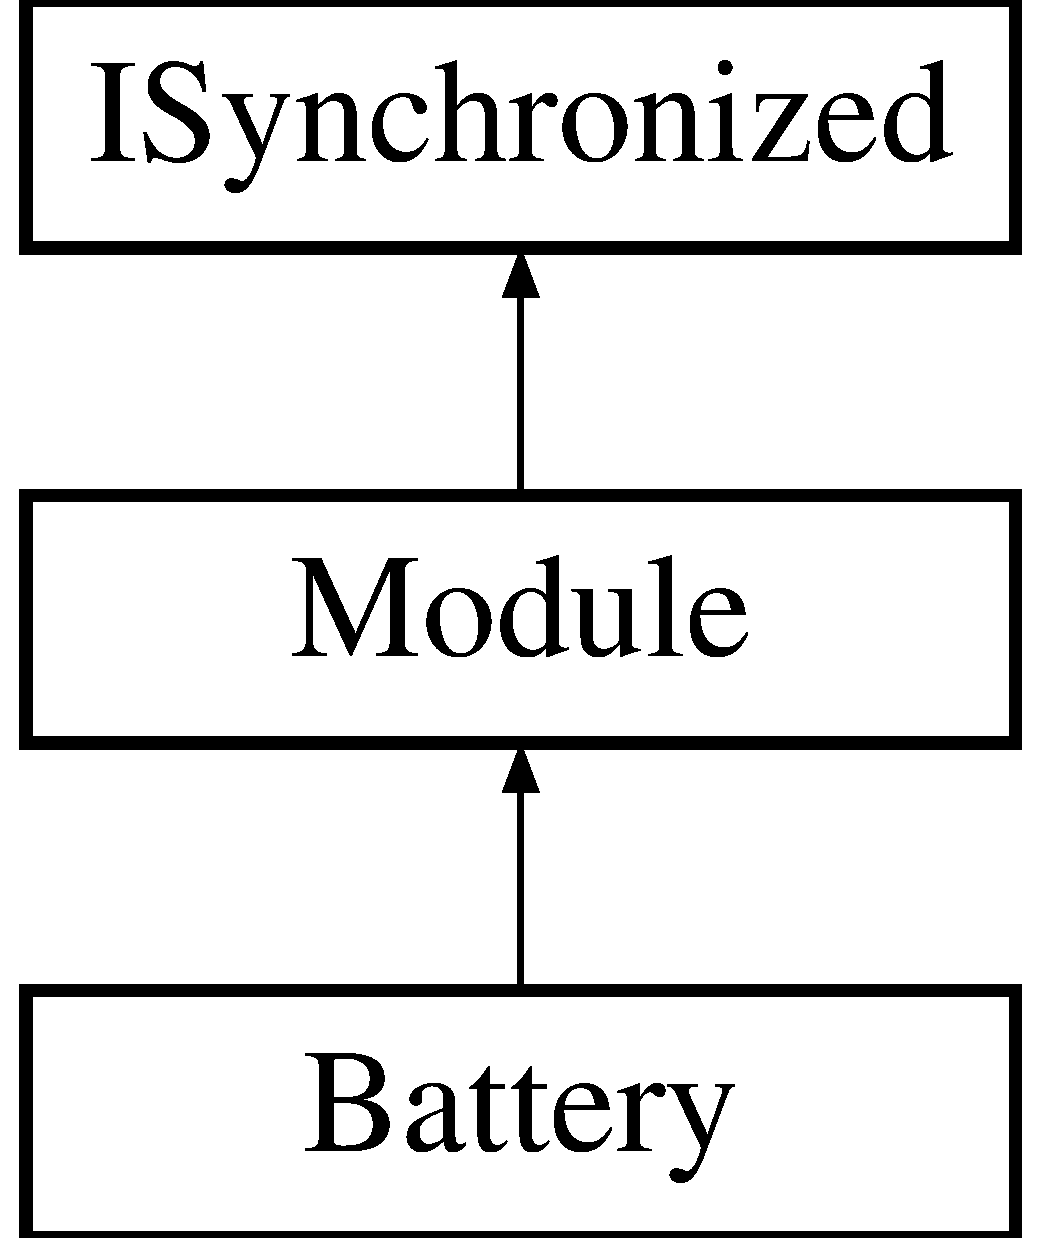
\includegraphics[height=3.000000cm]{classBattery}
\end{center}
\end{figure}
\subsection*{Fonctions membres publiques}
\begin{DoxyCompactItemize}
\item 
\hypertarget{classBattery_a2d41baf862c216d64f7455934422431b}{{\bfseries Battery} (Params=Params())}\label{classBattery_a2d41baf862c216d64f7455934422431b}

\end{DoxyCompactItemize}
\subsection*{Additional Inherited Members}


La documentation de cette classe a été générée à partir des fichiers suivants \-:\begin{DoxyCompactItemize}
\item 
src/\-Battery\-Module/Battery.\-h\item 
src/\-Battery\-Module/Battery.\-cpp\end{DoxyCompactItemize}

\hypertarget{classBatteryController}{\section{Référence de la classe Battery\-Controller}
\label{classBatteryController}\index{Battery\-Controller@{Battery\-Controller}}
}
Graphe d'héritage de Battery\-Controller\-:\begin{figure}[H]
\begin{center}
\leavevmode
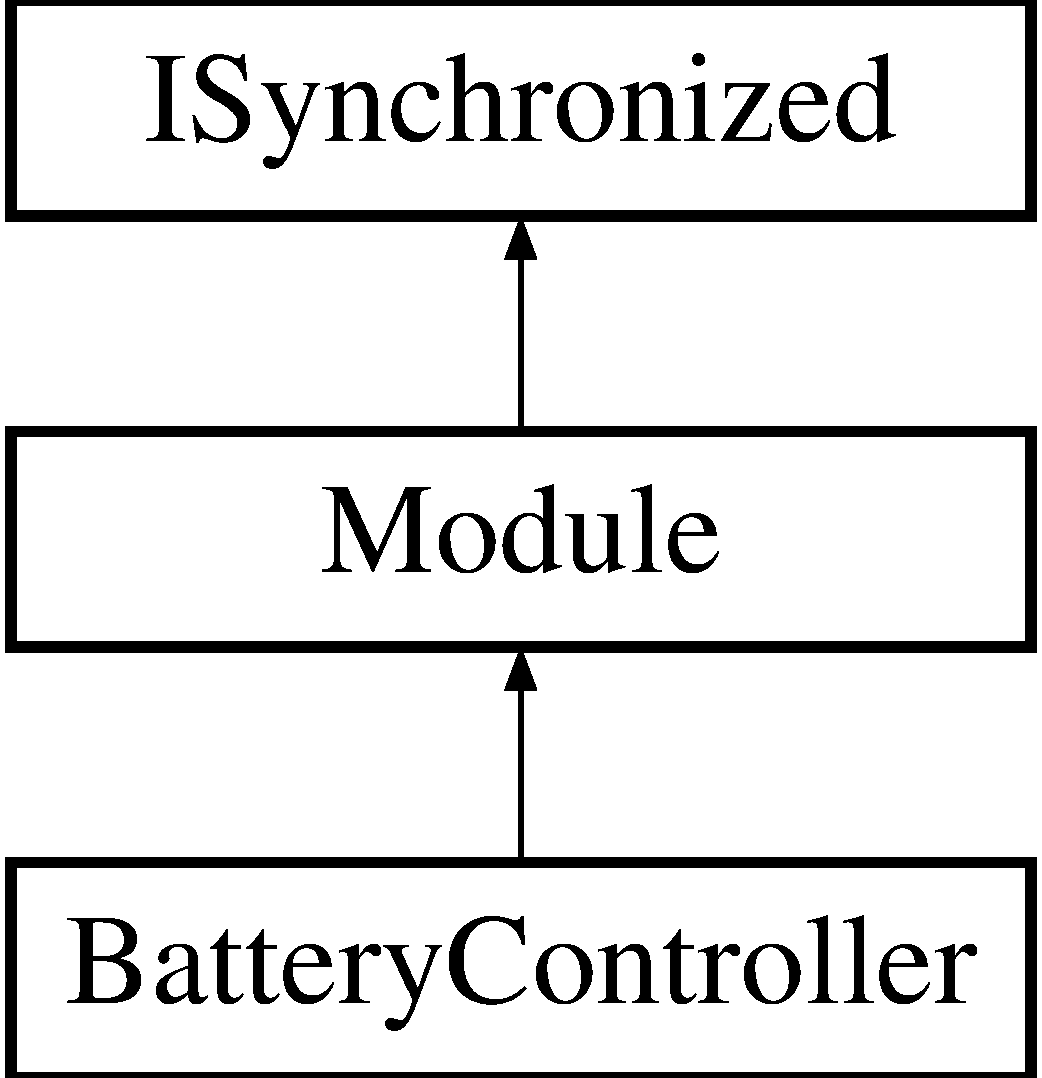
\includegraphics[height=3.000000cm]{classBatteryController}
\end{center}
\end{figure}
\subsection*{Fonctions membres publiques}
\begin{DoxyCompactItemize}
\item 
\hypertarget{classBatteryController_a48f46e2aa8ffb576634cdcb0ae172227}{{\bfseries Battery\-Controller} (Params=Params())}\label{classBatteryController_a48f46e2aa8ffb576634cdcb0ae172227}

\end{DoxyCompactItemize}
\subsection*{Additional Inherited Members}


La documentation de cette classe a été générée à partir des fichiers suivants \-:\begin{DoxyCompactItemize}
\item 
src/\-Battery\-Module/Battery\-Controller.\-h\item 
src/\-Battery\-Module/Battery\-Controller.\-cpp\end{DoxyCompactItemize}

\hypertarget{classBatteryModule}{\section{Référence de la classe Battery\-Module}
\label{classBatteryModule}\index{Battery\-Module@{Battery\-Module}}
}


Un exemple de batterie.  




{\ttfamily \#include $<$Battery\-Module.\-h$>$}

Graphe d'héritage de Battery\-Module\-:\begin{figure}[H]
\begin{center}
\leavevmode
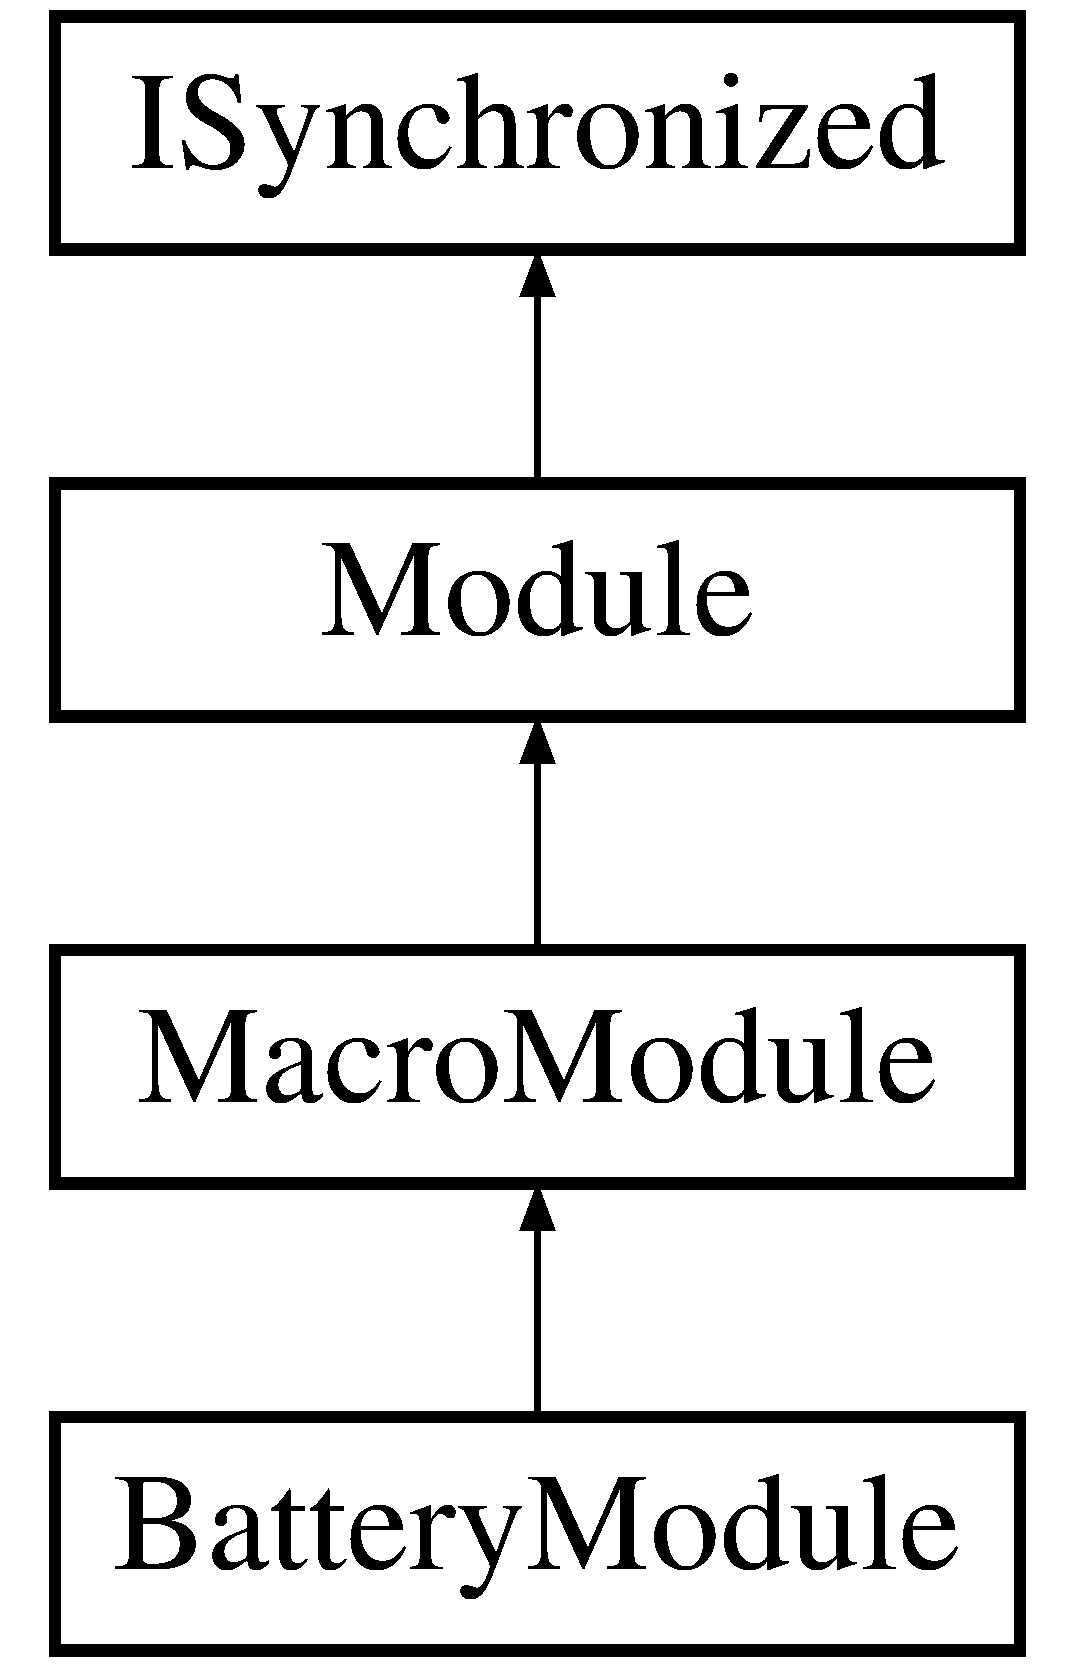
\includegraphics[height=4.000000cm]{classBatteryModule}
\end{center}
\end{figure}
\subsection*{Fonctions membres publiques}
\begin{DoxyCompactItemize}
\item 
\hyperlink{classBatteryModule_a2fb494ef5f124c38c0fdf9ccfb31918f}{Battery\-Module} (std\-::string \hyperlink{classModule_a794fbb44972c7c73cc197159093e66d1}{name}, Params params=Params())
\end{DoxyCompactItemize}
\subsection*{Membres hérités additionnels}


\subsection{Description détaillée}
Un exemple de batterie. 

On considère la batterie constituée de deux composants\-: la batterie en elle même, et son controlleur. Ceci est donc le macromodule qui les réunit. 

\subsection{Documentation des constructeurs et destructeur}
\hypertarget{classBatteryModule_a2fb494ef5f124c38c0fdf9ccfb31918f}{\index{Battery\-Module@{Battery\-Module}!Battery\-Module@{Battery\-Module}}
\index{Battery\-Module@{Battery\-Module}!BatteryModule@{Battery\-Module}}
\subsubsection[{Battery\-Module}]{\setlength{\rightskip}{0pt plus 5cm}Battery\-Module\-::\-Battery\-Module (
\begin{DoxyParamCaption}
\item[{std\-::string}]{name, }
\item[{Params}]{params = {\ttfamily Params()}}
\end{DoxyParamCaption}
)}}\label{classBatteryModule_a2fb494ef5f124c38c0fdf9ccfb31918f}
\begin{DoxyRefDesc}{A faire}
\item[\hyperlink{todo__todo000002}{A faire}]Surcharger \mbox{[}\mbox{]} pour getsocketbyname \end{DoxyRefDesc}


La documentation de cette classe a été générée à partir des fichiers suivants \-:\begin{DoxyCompactItemize}
\item 
src/\-Battery\-Module/Battery\-Module.\-h\item 
src/\-Battery\-Module/Battery\-Module.\-cpp\end{DoxyCompactItemize}

\hypertarget{classBatteryPhysics}{\section{Référence de la classe Battery\-Physics}
\label{classBatteryPhysics}\index{Battery\-Physics@{Battery\-Physics}}
}
Graphe d'héritage de Battery\-Physics\-:\begin{figure}[H]
\begin{center}
\leavevmode
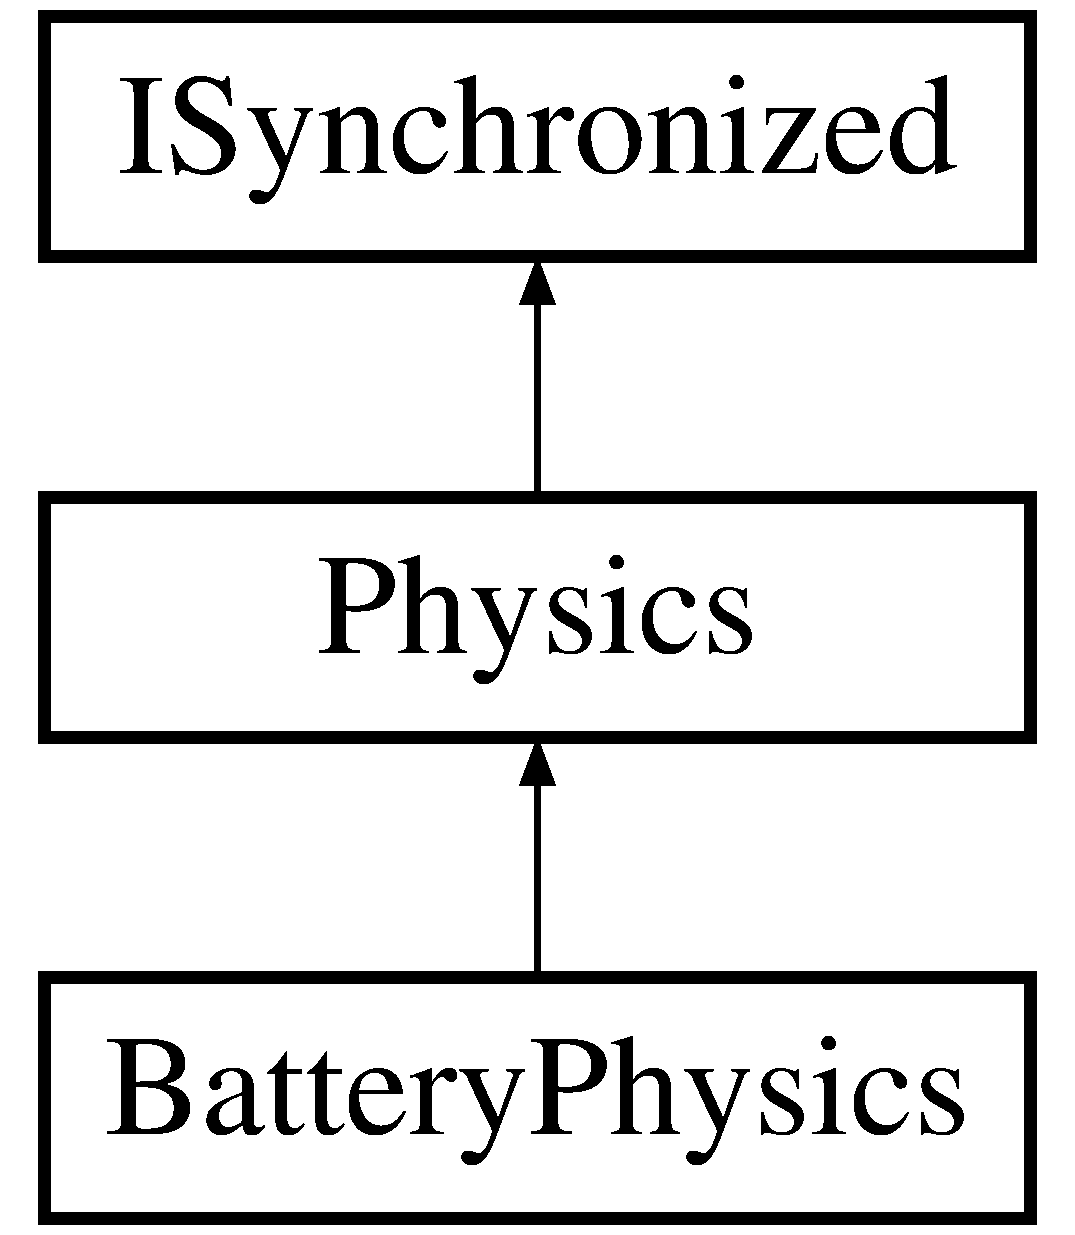
\includegraphics[height=3.000000cm]{classBatteryPhysics}
\end{center}
\end{figure}
\subsection*{Fonctions membres publiques}
\begin{DoxyCompactItemize}
\item 
\hypertarget{classBatteryPhysics_ac6fa6a615d95447a246d8f0dc01e7b02}{{\bfseries Battery\-Physics} (std\-::shared\-\_\-ptr$<$ \hyperlink{classModule}{Module} $>$)}\label{classBatteryPhysics_ac6fa6a615d95447a246d8f0dc01e7b02}

\item 
\hypertarget{classBatteryPhysics_a3651cc1fbb0d314a03d25af655804acc}{void \hyperlink{classBatteryPhysics_a3651cc1fbb0d314a03d25af655804acc}{clock} (int t)}\label{classBatteryPhysics_a3651cc1fbb0d314a03d25af655804acc}

\begin{DoxyCompactList}\small\item\em Méthode appellée à chaque pas de temps. \end{DoxyCompactList}\end{DoxyCompactItemize}
\subsection*{Membres hérités additionnels}


La documentation de cette classe a été générée à partir des fichiers suivants \-:\begin{DoxyCompactItemize}
\item 
src/\-Battery\-Module/Battery\-Physics.\-h\item 
src/\-Battery\-Module/Battery\-Physics.\-cpp\end{DoxyCompactItemize}

\hypertarget{classCLI}{\section{Référence de la classe C\-L\-I}
\label{classCLI}\index{C\-L\-I@{C\-L\-I}}
}
Graphe d'héritage de C\-L\-I\-:\begin{figure}[H]
\begin{center}
\leavevmode
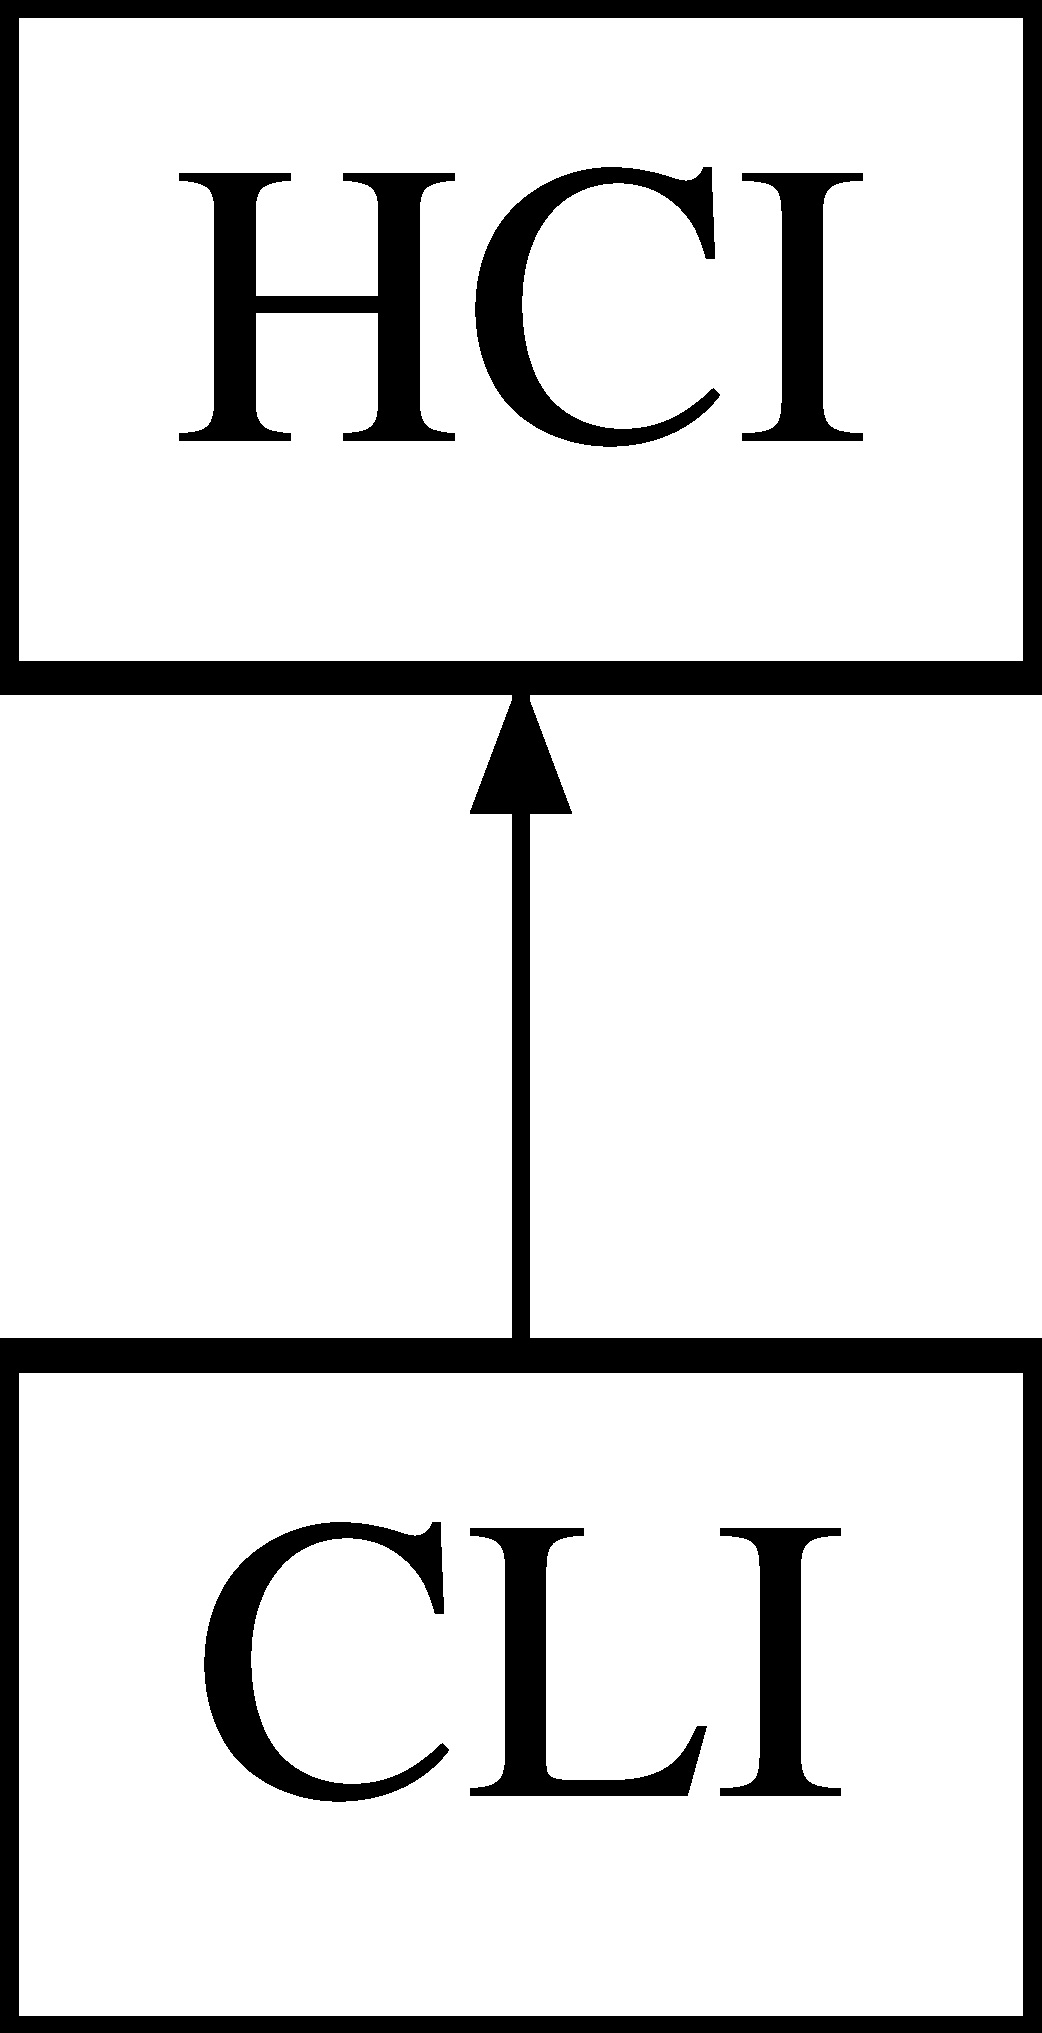
\includegraphics[height=2.000000cm]{classCLI}
\end{center}
\end{figure}
\subsection*{Fonctions membres publiques}
\begin{DoxyCompactItemize}
\item 
\hypertarget{classCLI_a43ec846cf90e311e7867d4315d4e559c}{void {\bfseries logv} (std\-::string, bool with\-Time=true) const }\label{classCLI_a43ec846cf90e311e7867d4315d4e559c}

\end{DoxyCompactItemize}
\subsection*{Fonctions membres publiques statiques}
\begin{DoxyCompactItemize}
\item 
\hypertarget{classCLI_afb0099de9473ff74480fa40cec78a3ac}{static \hyperlink{classCLI}{C\-L\-I} \& \hyperlink{classCLI_afb0099de9473ff74480fa40cec78a3ac}{get\-Instance} ()}\label{classCLI_afb0099de9473ff74480fa40cec78a3ac}

\begin{DoxyCompactList}\small\item\em Retourne l'instance unique de \hyperlink{classCLI}{C\-L\-I}. \end{DoxyCompactList}\end{DoxyCompactItemize}
\subsection*{Additional Inherited Members}


La documentation de cette classe a été générée à partir des fichiers suivants \-:\begin{DoxyCompactItemize}
\item 
src/\-Core/C\-L\-I.\-h\item 
src/\-Core/C\-L\-I.\-cpp\end{DoxyCompactItemize}

\hypertarget{classConnexion}{\section{Référence de la classe Connexion}
\label{classConnexion}\index{Connexion@{Connexion}}
}


Cette classe représente les tuyaux qui relient les \hyperlink{classSocket}{Socket}.  




{\ttfamily \#include $<$Connexion.\-h$>$}

\subsection*{Fonctions membres publiques}
\begin{DoxyCompactItemize}
\item 
\hyperlink{classConnexion_a31fda5acfafb5ec2de7ae76cfce373a7}{Connexion} (\hyperlink{classSocket}{Socket} $\ast$a, \hyperlink{classSocket}{Socket} $\ast$b)
\begin{DoxyCompactList}\small\item\em Constructeur, on créé une nouvelle connexion entre deux sockets en les informant mutuellement de leur compagnon (d'infortune ?). \end{DoxyCompactList}\item 
\hypertarget{classConnexion_a72dc9b8799eed7b02b7e75e8bccb601c}{{\bfseries Connexion} (const \hyperlink{classConnexion}{Connexion} \&)}\label{classConnexion_a72dc9b8799eed7b02b7e75e8bccb601c}

\item 
\hypertarget{classConnexion_a6afee761c33e160c2be5e9e2713968e3}{\hyperlink{classConnexion_a6afee761c33e160c2be5e9e2713968e3}{$\sim$\-Connexion} ()}\label{classConnexion_a6afee761c33e160c2be5e9e2713968e3}

\begin{DoxyCompactList}\small\item\em Destructeur. \end{DoxyCompactList}\item 
\hypertarget{classConnexion_ad39eca0322a2a8a49de21fdd910ea0db}{void \hyperlink{classConnexion_ad39eca0322a2a8a49de21fdd910ea0db}{dispatch} (std\-::shared\-\_\-ptr$<$ \hyperlink{classMessage}{Message} $>$, \hyperlink{classSocket}{Socket} $\ast$) const }\label{classConnexion_ad39eca0322a2a8a49de21fdd910ea0db}

\begin{DoxyCompactList}\small\item\em Envoie un message m d'un socket s vers son destinataire. \end{DoxyCompactList}\end{DoxyCompactItemize}


\subsection{Description détaillée}
Cette classe représente les tuyaux qui relient les \hyperlink{classSocket}{Socket}. 

\subsection{Documentation des constructeurs et destructeur}
\hypertarget{classConnexion_a31fda5acfafb5ec2de7ae76cfce373a7}{\index{Connexion@{Connexion}!Connexion@{Connexion}}
\index{Connexion@{Connexion}!Connexion@{Connexion}}
\subsubsection[{Connexion}]{\setlength{\rightskip}{0pt plus 5cm}Connexion\-::\-Connexion (
\begin{DoxyParamCaption}
\item[{{\bf Socket} $\ast$}]{a, }
\item[{{\bf Socket} $\ast$}]{b}
\end{DoxyParamCaption}
)}}\label{classConnexion_a31fda5acfafb5ec2de7ae76cfce373a7}


Constructeur, on créé une nouvelle connexion entre deux sockets en les informant mutuellement de leur compagnon (d'infortune ?). 

Constructeurpar copie. 

La documentation de cette classe a été générée à partir des fichiers suivants \-:\begin{DoxyCompactItemize}
\item 
src/\-Core/Connexion.\-h\item 
src/\-Core/Connexion.\-cpp\end{DoxyCompactItemize}

\hypertarget{classFloatMessage}{\section{Référence de la classe Float\-Message}
\label{classFloatMessage}\index{Float\-Message@{Float\-Message}}
}


Classe de messages contenant un nombre à virgule flottante comme le payload.  




{\ttfamily \#include $<$Float\-Message.\-h$>$}

Graphe d'héritage de Float\-Message\-:\begin{figure}[H]
\begin{center}
\leavevmode
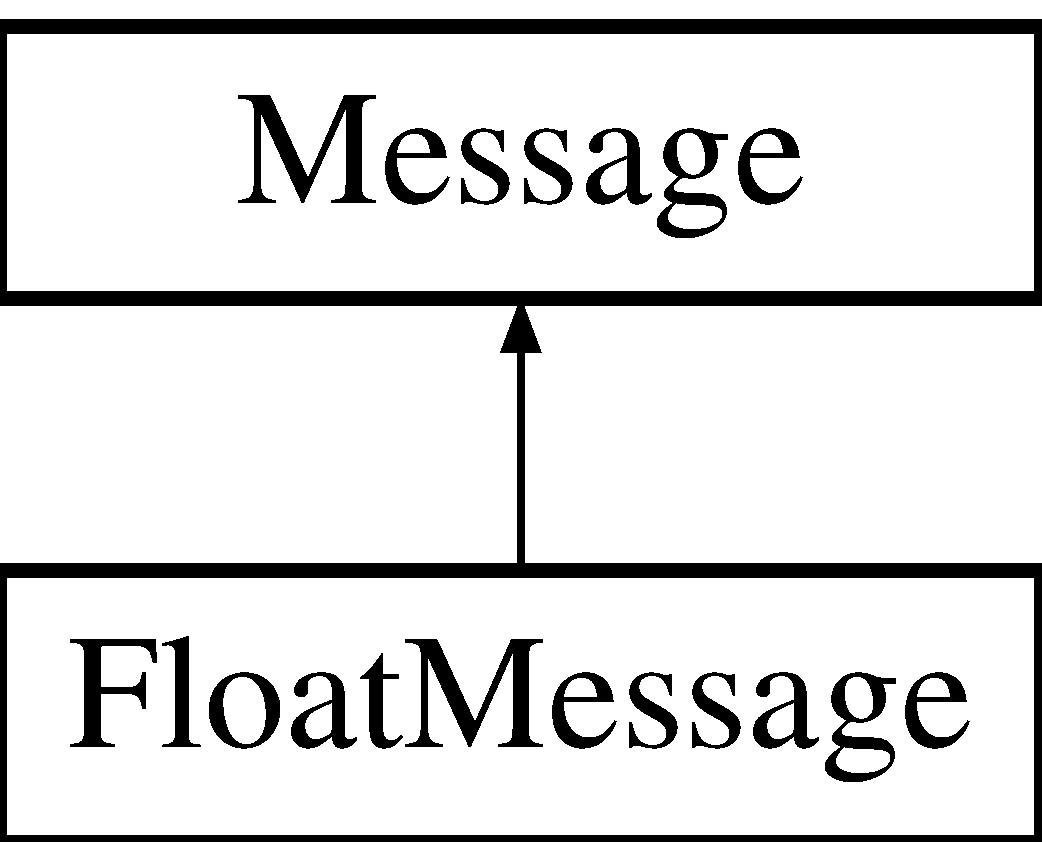
\includegraphics[height=2.000000cm]{classFloatMessage}
\end{center}
\end{figure}
\subsection*{Fonctions membres publiques}
\begin{DoxyCompactItemize}
\item 
\hypertarget{classFloatMessage_afad013afd6c0a51064e3df019c2ec6a5}{{\bfseries Float\-Message} (std\-::string \hyperlink{classMessage_ac7adddb666acdc47c48f684bd6810a51}{name}, float payload, int time=0)}\label{classFloatMessage_afad013afd6c0a51064e3df019c2ec6a5}

\item 
\hypertarget{classFloatMessage_a9b3814111c4194bc64a14f51dc4d10ce}{float \hyperlink{classFloatMessage_a9b3814111c4194bc64a14f51dc4d10ce}{get\-Payload} ()}\label{classFloatMessage_a9b3814111c4194bc64a14f51dc4d10ce}

\begin{DoxyCompactList}\small\item\em Renvoie la charge utile du message. \end{DoxyCompactList}\item 
\hypertarget{classFloatMessage_a8522c594c26e327e92546913d4ab4f4a}{std\-::ostream \& \hyperlink{classFloatMessage_a8522c594c26e327e92546913d4ab4f4a}{operator$<$$<$} (std\-::ostream \&os)}\label{classFloatMessage_a8522c594c26e327e92546913d4ab4f4a}

\begin{DoxyCompactList}\small\item\em Operateur de sortie surchargé \end{DoxyCompactList}\end{DoxyCompactItemize}
\subsection*{Membres hérités additionnels}


\subsection{Description détaillée}
Classe de messages contenant un nombre à virgule flottante comme le payload. 

La documentation de cette classe a été générée à partir des fichiers suivants \-:\begin{DoxyCompactItemize}
\item 
src/\-Core/\-Messages/Float\-Message.\-h\item 
src/\-Core/\-Messages/Float\-Message.\-cpp\end{DoxyCompactItemize}

\hypertarget{classHCI}{\section{Référence de la classe H\-C\-I}
\label{classHCI}\index{H\-C\-I@{H\-C\-I}}
}
Graphe d'héritage de H\-C\-I\-:\begin{figure}[H]
\begin{center}
\leavevmode
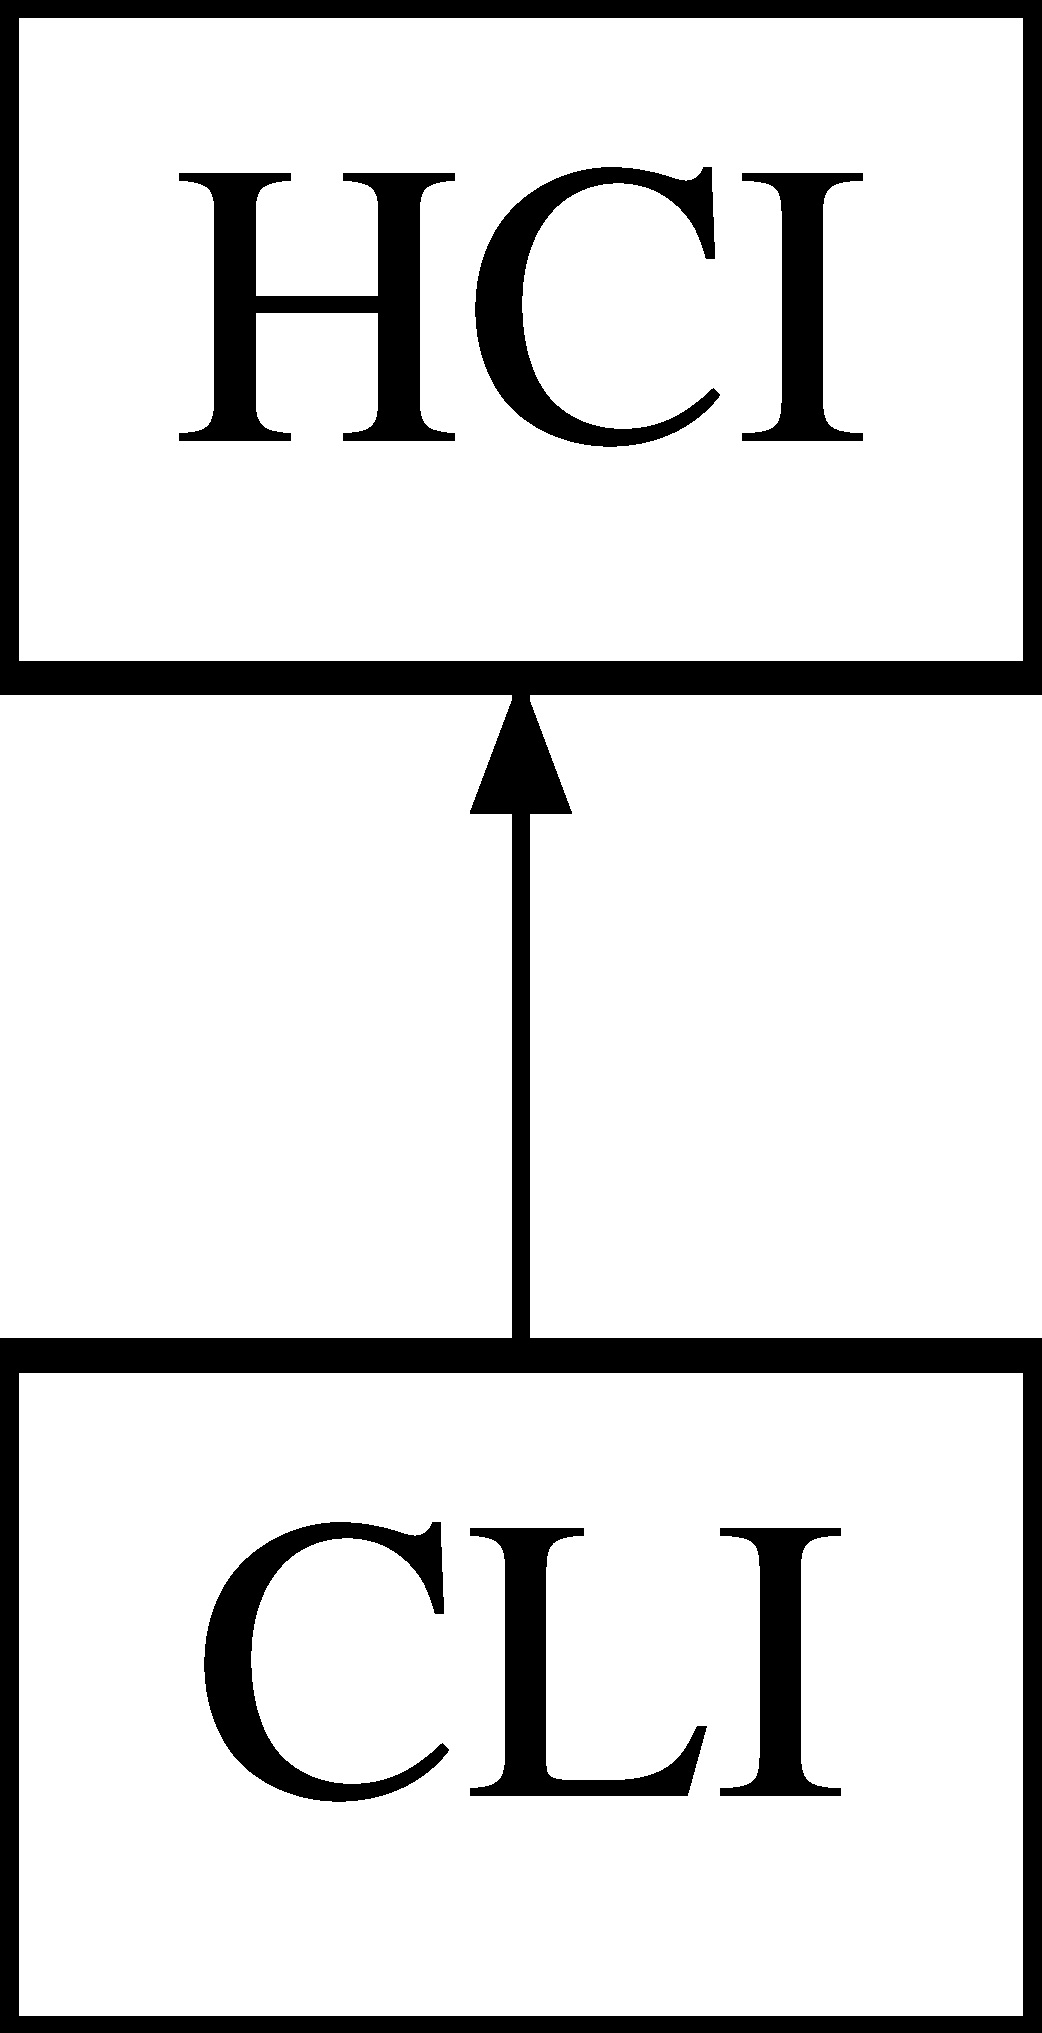
\includegraphics[height=2.000000cm]{classHCI}
\end{center}
\end{figure}
\subsection*{Types publics}
\begin{DoxyCompactItemize}
\item 
enum {\bfseries log\-Level} \{ \\*
{\bfseries N\-O\-T\-H\-I\-N\-G} =  -\/1, 
{\bfseries E\-R\-R\-O\-R} =  0, 
{\bfseries W\-A\-R\-N\-I\-N\-G} =  1, 
{\bfseries C\-R\-I\-T\-I\-N\-F\-O} =  2, 
\\*
{\bfseries I\-N\-F\-O} =  3
 \}
\end{DoxyCompactItemize}
\subsection*{Fonctions membres publiques}
\begin{DoxyCompactItemize}
\item 
\hypertarget{classHCI_a3cac51013396bb8a130298a04b966856}{{\bfseries H\-C\-I} (log\-Level=I\-N\-F\-O)}\label{classHCI_a3cac51013396bb8a130298a04b966856}

\item 
\hypertarget{classHCI_ab30b1bd8e7b5ddb8764128e9da1b3062}{void {\bfseries set\-Log\-Level} (log\-Level)}\label{classHCI_ab30b1bd8e7b5ddb8764128e9da1b3062}

\item 
\hypertarget{classHCI_a3ba0116597c8a43a7ceac9639150e6c1}{void {\bfseries log} (log\-Level, std\-::string, bool with\-Time=true) const }\label{classHCI_a3ba0116597c8a43a7ceac9639150e6c1}

\item 
\hypertarget{classHCI_a63e5f2061611136d467cda53e4636713}{virtual void {\bfseries logv} (std\-::string, bool with\-Time) const =0}\label{classHCI_a63e5f2061611136d467cda53e4636713}

\end{DoxyCompactItemize}
\subsection*{Attributs protégés}
\begin{DoxyCompactItemize}
\item 
\hypertarget{classHCI_ac344060f03fa9aa1809cfecb507a83f9}{log\-Level {\bfseries log\-Lev}}\label{classHCI_ac344060f03fa9aa1809cfecb507a83f9}

\end{DoxyCompactItemize}


La documentation de cette classe a été générée à partir des fichiers suivants \-:\begin{DoxyCompactItemize}
\item 
src/\-Core/H\-C\-I.\-h\item 
src/\-Core/H\-C\-I.\-cpp\end{DoxyCompactItemize}

\hypertarget{classIntMessage}{\section{Référence de la classe Int\-Message}
\label{classIntMessage}\index{Int\-Message@{Int\-Message}}
}


Classe de messages contenant entier comme le payload.  




{\ttfamily \#include $<$Int\-Message.\-h$>$}

Graphe d'héritage de Int\-Message\-:\begin{figure}[H]
\begin{center}
\leavevmode
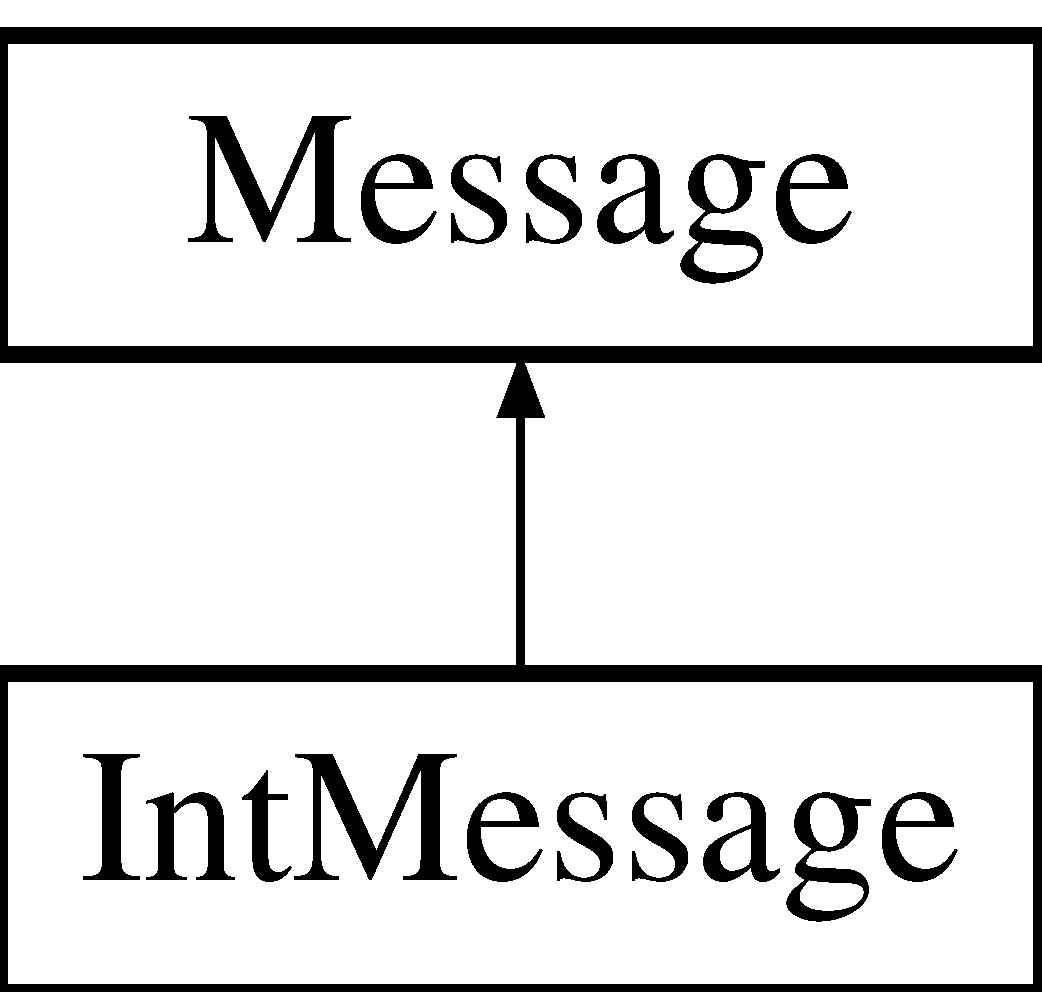
\includegraphics[height=2.000000cm]{classIntMessage}
\end{center}
\end{figure}
\subsection*{Fonctions membres publiques}
\begin{DoxyCompactItemize}
\item 
\hypertarget{classIntMessage_aae52ad3c838b48d6512eea7ffbb89404}{{\bfseries Int\-Message} (std\-::string \hyperlink{classMessage_ac7adddb666acdc47c48f684bd6810a51}{name}, int payload, int time=0)}\label{classIntMessage_aae52ad3c838b48d6512eea7ffbb89404}

\item 
\hypertarget{classIntMessage_a00d3fe88985495e98725c12bfc21c39d}{int \hyperlink{classIntMessage_a00d3fe88985495e98725c12bfc21c39d}{get\-Payload} ()}\label{classIntMessage_a00d3fe88985495e98725c12bfc21c39d}

\begin{DoxyCompactList}\small\item\em Renvoie la charge utile du message. \end{DoxyCompactList}\item 
\hypertarget{classIntMessage_a222a5ba75846757bfc24cea19ce345ed}{std\-::ostream \& \hyperlink{classIntMessage_a222a5ba75846757bfc24cea19ce345ed}{operator$<$$<$} (std\-::ostream \&os)}\label{classIntMessage_a222a5ba75846757bfc24cea19ce345ed}

\begin{DoxyCompactList}\small\item\em Operateur de sortie surchargé \end{DoxyCompactList}\end{DoxyCompactItemize}
\subsection*{Membres hérités additionnels}


\subsection{Description détaillée}
Classe de messages contenant entier comme le payload. 

La documentation de cette classe a été générée à partir des fichiers suivants \-:\begin{DoxyCompactItemize}
\item 
src/\-Core/\-Messages/Int\-Message.\-h\item 
src/\-Core/\-Messages/Int\-Message.\-cpp\end{DoxyCompactItemize}

\hypertarget{classISynchronized}{\section{Référence de la classe I\-Synchronized}
\label{classISynchronized}\index{I\-Synchronized@{I\-Synchronized}}
}


Interface pour ÈlÈment synchronisÈ  




{\ttfamily \#include $<$I\-Synchronized.\-h$>$}

Graphe d'héritage de I\-Synchronized\-:\begin{figure}[H]
\begin{center}
\leavevmode
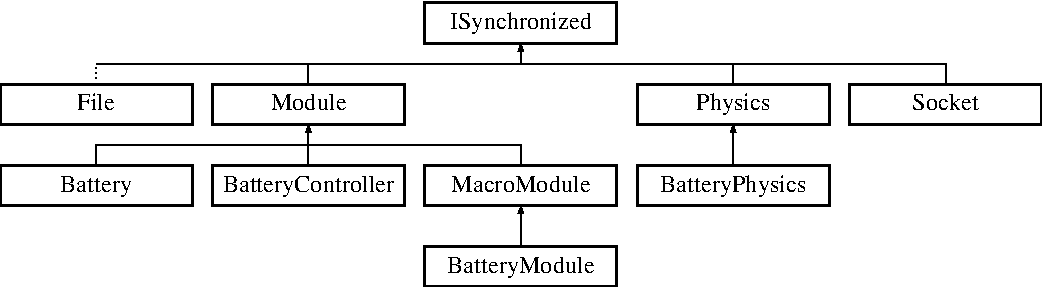
\includegraphics[height=4.000000cm]{classISynchronized}
\end{center}
\end{figure}
\subsection*{Fonctions membres publiques}
\begin{DoxyCompactItemize}
\item 
\hypertarget{classISynchronized_af7155c662758d6c70f381bb9b11afcd6}{virtual void \hyperlink{classISynchronized_af7155c662758d6c70f381bb9b11afcd6}{clock} (int time)=0}\label{classISynchronized_af7155c662758d6c70f381bb9b11afcd6}

\begin{DoxyCompactList}\small\item\em Methode appellé à chaque tick d'horloge liée. \end{DoxyCompactList}\end{DoxyCompactItemize}


\subsection{Description détaillée}
Interface pour ÈlÈment synchronisÈ 

Cette interface vise ‡ homogÈnÈiser la notion de temps (timer) pour les classes qui en dÈpendent. 

La documentation de cette classe a été générée à partir du fichier suivant \-:\begin{DoxyCompactItemize}
\item 
src/headers/I\-Synchronized.\-h\end{DoxyCompactItemize}

\hypertarget{classMacroModule}{\section{Référence de la classe Macro\-Module}
\label{classMacroModule}\index{Macro\-Module@{Macro\-Module}}
}
Graphe d'héritage de Macro\-Module\-:\begin{figure}[H]
\begin{center}
\leavevmode
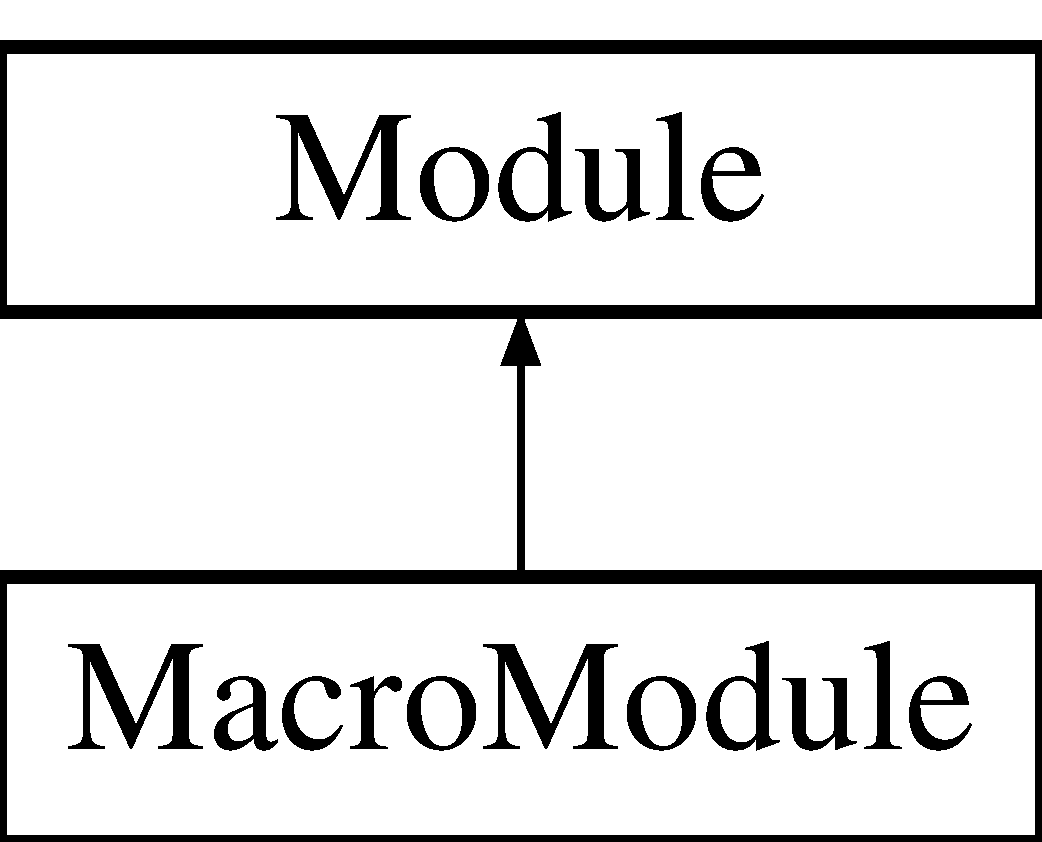
\includegraphics[height=4.000000cm]{classMacroModule}
\end{center}
\end{figure}
\subsection*{Fonctions membres publiques}
\begin{DoxyCompactItemize}
\item 
\hypertarget{classMacroModule_a9a7fef08bb03b97cb018b4cd7ad95c64}{{\bfseries Macro\-Module} (std\-::string=\char`\"{}Default\-Name\char`\"{}, Params=Params(), std\-::string cp=std\-::string())}\label{classMacroModule_a9a7fef08bb03b97cb018b4cd7ad95c64}

\item 
\hypertarget{classMacroModule_aa7d592010b740d68028fee87e139ae9f}{\hyperlink{classMacroModule_aa7d592010b740d68028fee87e139ae9f}{Macro\-Module} (std\-::string, \hyperlink{classMemory}{Memory}$<$ int $>$, Params=Params())}\label{classMacroModule_aa7d592010b740d68028fee87e139ae9f}

\begin{DoxyCompactList}\small\item\em Constructeur avec m�moire. \end{DoxyCompactList}\item 
\hypertarget{classMacroModule_a9790fb7c331d99dd03f624b1a5258519}{virtual \hyperlink{classMacroModule_a9790fb7c331d99dd03f624b1a5258519}{$\sim$\-Macro\-Module} ()}\label{classMacroModule_a9790fb7c331d99dd03f624b1a5258519}

\begin{DoxyCompactList}\small\item\em Destructeur. \end{DoxyCompactList}\item 
\hypertarget{classMacroModule_a3c693014fb5e1a46758e7867eca43342}{void \hyperlink{classMacroModule_a3c693014fb5e1a46758e7867eca43342}{add\-Sub\-Module} (\hyperlink{classModule}{Module} $\ast$)}\label{classMacroModule_a3c693014fb5e1a46758e7867eca43342}

\begin{DoxyCompactList}\small\item\em Ajoute un sous-\/module � la liste. \end{DoxyCompactList}\item 
\hypertarget{classMacroModule_a6ad4d6abd8bb4b742b800f6fa3c98296}{void \hyperlink{classMacroModule_a6ad4d6abd8bb4b742b800f6fa3c98296}{add\-Connexion} (\hyperlink{classConnexion}{Connexion} $\ast$)}\label{classMacroModule_a6ad4d6abd8bb4b742b800f6fa3c98296}

\begin{DoxyCompactList}\small\item\em Ajoute une connexion � la liste. \end{DoxyCompactList}\item 
\hypertarget{classMacroModule_ab98b15af55e4cd1ad3a20fc53af09aa4}{std\-::shared\-\_\-ptr$<$ \hyperlink{classModule}{Module} $>$ \hyperlink{classMacroModule_ab98b15af55e4cd1ad3a20fc53af09aa4}{get\-Module\-By\-Name} (std\-::string)}\label{classMacroModule_ab98b15af55e4cd1ad3a20fc53af09aa4}

\begin{DoxyCompactList}\small\item\em Renvoie le module voulu Exception g�r�e. \end{DoxyCompactList}\end{DoxyCompactItemize}
\subsection*{Additional Inherited Members}


La documentation de cette classe a été générée à partir des fichiers suivants \-:\begin{DoxyCompactItemize}
\item 
src/\-Core/Macro\-Module.\-h\item 
src/\-Core/Macro\-Module.\-cpp\end{DoxyCompactItemize}

\hypertarget{classMemory}{\section{Référence du modèle de la classe Memory$<$ T $>$}
\label{classMemory}\index{Memory$<$ T $>$@{Memory$<$ T $>$}}
}


Représente une mémoire.  




{\ttfamily \#include $<$Memory.\-h$>$}

\subsection*{Fonctions membres publiques}
\begin{DoxyCompactItemize}
\item 
\hypertarget{classMemory_aa546b7c6e170e45a4e4f74492d8fe8bf}{\hyperlink{classMemory_aa546b7c6e170e45a4e4f74492d8fe8bf}{Memory} ()}\label{classMemory_aa546b7c6e170e45a4e4f74492d8fe8bf}

\begin{DoxyCompactList}\small\item\em Constructeur. \end{DoxyCompactList}\item 
\hypertarget{classMemory_af1e6452dbe3bb1650604140814710b95}{\hyperlink{classMemory_af1e6452dbe3bb1650604140814710b95}{Memory} (std\-::unordered\-\_\-map$<$ std\-::string, T $>$)}\label{classMemory_af1e6452dbe3bb1650604140814710b95}

\begin{DoxyCompactList}\small\item\em Constructeur parametrisé avec cells. \end{DoxyCompactList}\item 
\hypertarget{classMemory_add46d3ed56cf1e88efee2ed59b38c995}{unsigned int \hyperlink{classMemory_add46d3ed56cf1e88efee2ed59b38c995}{get\-Size} ()}\label{classMemory_add46d3ed56cf1e88efee2ed59b38c995}

\begin{DoxyCompactList}\small\item\em Retourne la taille courante de la mémoire. \end{DoxyCompactList}\item 
\hypertarget{classMemory_a3514e7594615bb1748ba5b57259c9eca}{int \hyperlink{classMemory_a3514e7594615bb1748ba5b57259c9eca}{set\-Value\-For\-Key} (std\-::string, T)}\label{classMemory_a3514e7594615bb1748ba5b57259c9eca}

\begin{DoxyCompactList}\small\item\em écrit une valeur \char`\"{}value\char`\"{} dans la case mémoire avec un nom \char`\"{}key\char`\"{}. \end{DoxyCompactList}\item 
\hypertarget{classMemory_a2d153fdede89954dc0875ab6c8d804c3}{\hyperlink{classMemory_a2d153fdede89954dc0875ab6c8d804c3}{$\sim$\-Memory} ()}\label{classMemory_a2d153fdede89954dc0875ab6c8d804c3}

\begin{DoxyCompactList}\small\item\em Destructeur. \end{DoxyCompactList}\end{DoxyCompactItemize}


\subsection{Description détaillée}
\subsubsection*{template$<$class T$>$class Memory$<$ T $>$}

Représente une mémoire. 

La mémoire est ici simplement modélisée comme une liste de clées et de valeurs, associée à des contraintes. 

La documentation de cette classe a été générée à partir des fichiers suivants \-:\begin{DoxyCompactItemize}
\item 
src/\-Core/Memory.\-h\item 
src/\-Core/Memory.\-cpp\end{DoxyCompactItemize}

\hypertarget{classMessage}{\section{Référence de la classe Message}
\label{classMessage}\index{Message@{Message}}
}


Classe abstraite de base pour les messages.  




{\ttfamily \#include $<$Message.\-h$>$}

Graphe d'héritage de Message\-:\begin{figure}[H]
\begin{center}
\leavevmode
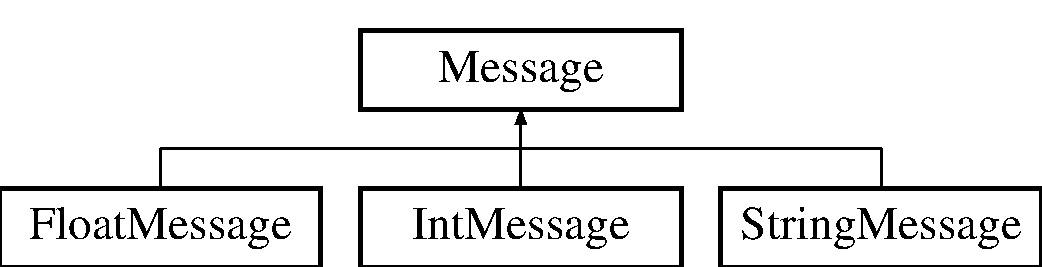
\includegraphics[height=2.000000cm]{classMessage}
\end{center}
\end{figure}
\subsection*{Fonctions membres publiques}
\begin{DoxyCompactItemize}
\item 
\hypertarget{classMessage_a154809183fa5ec6b5182c487db1167dd}{\hyperlink{classMessage_a154809183fa5ec6b5182c487db1167dd}{Message} (std\-::string \hyperlink{classMessage_ac7adddb666acdc47c48f684bd6810a51}{name}=\char`\"{}Default Name\char`\"{}, int=0)}\label{classMessage_a154809183fa5ec6b5182c487db1167dd}

\begin{DoxyCompactList}\small\item\em Constructeur par défaut. \end{DoxyCompactList}\item 
\hypertarget{classMessage_a3f7275462831f787a861271687bcad67}{virtual \hyperlink{classMessage_a3f7275462831f787a861271687bcad67}{$\sim$\-Message} ()}\label{classMessage_a3f7275462831f787a861271687bcad67}

\begin{DoxyCompactList}\small\item\em Destructeur. \end{DoxyCompactList}\item 
\hypertarget{classMessage_ac03b02000572b0852c574498bf138e87}{std\-::string \hyperlink{classMessage_ac03b02000572b0852c574498bf138e87}{get\-Name} ()}\label{classMessage_ac03b02000572b0852c574498bf138e87}

\begin{DoxyCompactList}\small\item\em Renvoie le nom du message. \end{DoxyCompactList}\item 
\hypertarget{classMessage_acbdab136245666bce3752fa311150672}{virtual std\-::ostream \& \hyperlink{classMessage_acbdab136245666bce3752fa311150672}{operator$<$$<$} (std\-::ostream \&os)=0}\label{classMessage_acbdab136245666bce3752fa311150672}

\begin{DoxyCompactList}\small\item\em Operateur de sortie surchargé \end{DoxyCompactList}\item 
\hypertarget{classMessage_a37550fee6e64d7c83ead2628373f4db3}{unsigned int \hyperlink{classMessage_a37550fee6e64d7c83ead2628373f4db3}{get\-Transmission\-Time} ()}\label{classMessage_a37550fee6e64d7c83ead2628373f4db3}

\begin{DoxyCompactList}\small\item\em Renvoie le temps de traitement du message. \end{DoxyCompactList}\end{DoxyCompactItemize}
\subsection*{Fonctions membres publiques statiques}
\begin{DoxyCompactItemize}
\item 
\hypertarget{classMessage_a18fddc1357914aa65d4a12eeabbf7bfa}{static std\-::shared\-\_\-ptr$<$ \hyperlink{classMessage}{Message} $>$ {\bfseries create\-Message} (std\-::string, int=0, unsigned int=0)}\label{classMessage_a18fddc1357914aa65d4a12eeabbf7bfa}

\item 
\hypertarget{classMessage_a9510bbfbcde96a857eb40b8222fe90a8}{static std\-::shared\-\_\-ptr$<$ \hyperlink{classMessage}{Message} $>$ {\bfseries create\-Message} (std\-::string, std\-::string=\char`\"{}\char`\"{}, unsigned int=0)}\label{classMessage_a9510bbfbcde96a857eb40b8222fe90a8}

\item 
\hypertarget{classMessage_a275c24aa740943af5872d874eeca0173}{static std\-::shared\-\_\-ptr$<$ \hyperlink{classMessage}{Message} $>$ \hyperlink{classMessage_a275c24aa740943af5872d874eeca0173}{create\-Message} (std\-::string, float=0, unsigned=0)}\label{classMessage_a275c24aa740943af5872d874eeca0173}

\begin{DoxyCompactList}\small\item\em Crée et retourne le pointeur partagé au nouveau \hyperlink{classFloatMessage}{Float\-Message}. \end{DoxyCompactList}\end{DoxyCompactItemize}
\subsection*{Attributs protégés}
\begin{DoxyCompactItemize}
\item 
std\-::string \hyperlink{classMessage_ac7adddb666acdc47c48f684bd6810a51}{name}
\item 
unsigned int \hyperlink{classMessage_a9f2d70860e0ec546c8e00cd69a3555ee}{transmission\-Time}
\end{DoxyCompactItemize}


\subsection{Description détaillée}
Classe abstraite de base pour les messages. 

Les messages sont les différentes informations que peuvent se communiquer les modules. Un message est composé de son nom, éventuellement d'une donnée (payload), et d'une indication temporelle concernant la durée de son envoi et de sa réception. 

\subsection{Documentation des données membres}
\hypertarget{classMessage_ac7adddb666acdc47c48f684bd6810a51}{\index{Message@{Message}!name@{name}}
\index{name@{name}!Message@{Message}}
\subsubsection[{name}]{\setlength{\rightskip}{0pt plus 5cm}std\-::string Message\-::name\hspace{0.3cm}{\ttfamily [protected]}}}\label{classMessage_ac7adddb666acdc47c48f684bd6810a51}
Nom du message \hypertarget{classMessage_a9f2d70860e0ec546c8e00cd69a3555ee}{\index{Message@{Message}!transmission\-Time@{transmission\-Time}}
\index{transmission\-Time@{transmission\-Time}!Message@{Message}}
\subsubsection[{transmission\-Time}]{\setlength{\rightskip}{0pt plus 5cm}unsigned int Message\-::transmission\-Time\hspace{0.3cm}{\ttfamily [protected]}}}\label{classMessage_a9f2d70860e0ec546c8e00cd69a3555ee}
Temps de traitement du message 

La documentation de cette classe a été générée à partir des fichiers suivants \-:\begin{DoxyCompactItemize}
\item 
src/\-Core/Message.\-h\item 
src/\-Core/Message.\-cpp\end{DoxyCompactItemize}

\hypertarget{classModule}{\section{Référence de la classe Module}
\label{classModule}\index{Module@{Module}}
}


Les briques de base du simulateur.  




{\ttfamily \#include $<$Module.\-h$>$}

Graphe d'héritage de Module\-:\begin{figure}[H]
\begin{center}
\leavevmode
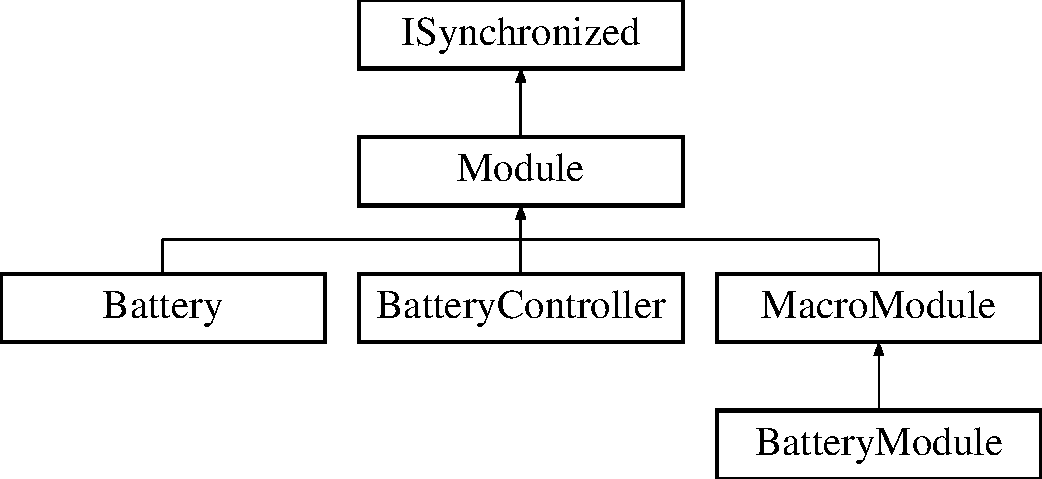
\includegraphics[height=4.000000cm]{classModule}
\end{center}
\end{figure}
\subsection*{Fonctions membres publiques}
\begin{DoxyCompactItemize}
\item 
\hypertarget{classModule_abcdd948c7444d3420f04be1bd332fbae}{\hyperlink{classModule_abcdd948c7444d3420f04be1bd332fbae}{Module} (std\-::string=\char`\"{}Default\-Name\char`\"{}, Params=Params(), std\-::string cp=std\-::string())}\label{classModule_abcdd948c7444d3420f04be1bd332fbae}

\begin{DoxyCompactList}\small\item\em Constructeur par défault, pour un module sans mémoire. \end{DoxyCompactList}\item 
\hypertarget{classModule_ae2ce24f11deec1453dfaba1f21a36f2c}{\hyperlink{classModule_ae2ce24f11deec1453dfaba1f21a36f2c}{Module} (std\-::string, \hyperlink{classMemory}{Memory}$<$ int $>$, Params=Params())}\label{classModule_ae2ce24f11deec1453dfaba1f21a36f2c}

\begin{DoxyCompactList}\small\item\em Constructeur avec mémoire. \end{DoxyCompactList}\item 
\hypertarget{classModule_a7c9d9c096786d127590fdd8aa2b7d681}{virtual \hyperlink{classModule_a7c9d9c096786d127590fdd8aa2b7d681}{$\sim$\-Module} ()}\label{classModule_a7c9d9c096786d127590fdd8aa2b7d681}

\begin{DoxyCompactList}\small\item\em Destructeur. \end{DoxyCompactList}\item 
virtual void \hyperlink{classModule_ab7ea9648fa500696c85e93ebd0666390}{clock} (int)
\begin{DoxyCompactList}\small\item\em Méthode appellée à chaque pas de temps, commune à tous les modules. \end{DoxyCompactList}\item 
\hypertarget{classModule_aeb7302c667eb923a4dc25ae235c744dc}{void \hyperlink{classModule_aeb7302c667eb923a4dc25ae235c744dc}{add\-Socket} (\hyperlink{classSocket}{Socket})}\label{classModule_aeb7302c667eb923a4dc25ae235c744dc}

\begin{DoxyCompactList}\small\item\em Fonction d'ajout d'un connecteur au module. \end{DoxyCompactList}\item 
\hypertarget{classModule_a146f454fded03cda14359e419086afa5}{void \hyperlink{classModule_a146f454fded03cda14359e419086afa5}{add\-Message} (std\-::string, int)}\label{classModule_a146f454fded03cda14359e419086afa5}

\begin{DoxyCompactList}\small\item\em Fonction d'ajout d'un message au module, et de son temps d'éxecution simulé. \end{DoxyCompactList}\item 
\hyperlink{classSocket}{Socket} $\ast$ \hyperlink{classModule_aed844ffed911793d3895c5a2bc4f9d43}{get\-Socket\-By\-Name} (std\-::string)
\begin{DoxyCompactList}\small\item\em Récupère le bon connecteur, ou lève une exception. \end{DoxyCompactList}\item 
\hypertarget{classModule_a93e2ee84587751939c1fd31cb0802e41}{double {\bfseries get\-Param\-Value\-By\-Name} (std\-::string)}\label{classModule_a93e2ee84587751939c1fd31cb0802e41}

\item 
\hypertarget{classModule_ace0e4299e1a6f9b46aa9fd316483895d}{void {\bfseries set\-Param\-Value\-By\-Name} (std\-::string, double)}\label{classModule_ace0e4299e1a6f9b46aa9fd316483895d}

\item 
\hypertarget{classModule_a6e425394cec58009568822cc7a09c8c1}{bool \hyperlink{classModule_a6e425394cec58009568822cc7a09c8c1}{is\-Message\-Allowed} (std\-::string)}\label{classModule_a6e425394cec58009568822cc7a09c8c1}

\begin{DoxyCompactList}\small\item\em Vérifie si le message est un des messages compris par ce module. \end{DoxyCompactList}\item 
\hypertarget{classModule_a3c1ecab9c7fa778807e253c26aa54310}{std\-::string \hyperlink{classModule_a3c1ecab9c7fa778807e253c26aa54310}{get\-Name} () const }\label{classModule_a3c1ecab9c7fa778807e253c26aa54310}

\begin{DoxyCompactList}\small\item\em Vérifie si le message est un des messages compris par ce module. \end{DoxyCompactList}\end{DoxyCompactItemize}
\subsection*{Attributs protégés}
\begin{DoxyCompactItemize}
\item 
std\-::string \hyperlink{classModule_a794fbb44972c7c73cc197159093e66d1}{name}
\item 
std\-::string \hyperlink{classModule_a5c7481c5ac746e01b225b6782e915dac}{conf\-Path}
\item 
\hyperlink{classMemory}{Memory}$<$ int $>$ \hyperlink{classModule_a48fa02fe55d33daffff725c615a63bb9}{memory}
\item 
Sockets \hyperlink{classModule_af0415ddaab230958f91665c66b078085}{sockets}
\item 
Messages \hyperlink{classModule_aaadd1f971bebf7bb5eae12fcc5689198}{messages\-Allowed}
\item 
Params \hyperlink{classModule_a232443111a9d59c17724992ddf75fbad}{parameters}
\item 
std\-::queue$<$ std\-::shared\-\_\-ptr\\*
$<$ \hyperlink{classMessage}{Message} $>$ $>$ \hyperlink{classModule_a93e833bd46e53a2d52ab63afb304b840}{tasks}
\item 
int \hyperlink{classModule_afc209c4f9120425219f7775c79cf4bea}{task\-Timer}
\end{DoxyCompactItemize}


\subsection{Description détaillée}
Les briques de base du simulateur. 

Il s'agit de la classe centrale du simulateur, qui sera construit comme un assemblage de modules qui communiquent entre eux. Il s'agit d'une classe virtuelle. Nécessitant un contrôle de la part du timer, elle implémente l'interface \hyperlink{classISynchronized}{I\-Synchronized} 

\subsection{Documentation des fonctions membres}
\hypertarget{classModule_ab7ea9648fa500696c85e93ebd0666390}{\index{Module@{Module}!clock@{clock}}
\index{clock@{clock}!Module@{Module}}
\subsubsection[{clock}]{\setlength{\rightskip}{0pt plus 5cm}void Module\-::clock (
\begin{DoxyParamCaption}
\item[{int}]{time}
\end{DoxyParamCaption}
)\hspace{0.3cm}{\ttfamily [virtual]}}}\label{classModule_ab7ea9648fa500696c85e93ebd0666390}


Méthode appellée à chaque pas de temps, commune à tous les modules. 

Cette méthode effectue trois actions, lire les messages arrivés, avancer dans un processus interne, envoyer un message. Ces actions prennent tous du temps\-: elles peuvent durer plusieurs \char`\"{}ticks\char`\"{}. \begin{DoxyRefDesc}{A faire}
\item[\hyperlink{todo__todo000005}{A faire}]Lever une exception \end{DoxyRefDesc}


Implémente \hyperlink{classISynchronized_af7155c662758d6c70f381bb9b11afcd6}{I\-Synchronized}.

\hypertarget{classModule_aed844ffed911793d3895c5a2bc4f9d43}{\index{Module@{Module}!get\-Socket\-By\-Name@{get\-Socket\-By\-Name}}
\index{get\-Socket\-By\-Name@{get\-Socket\-By\-Name}!Module@{Module}}
\subsubsection[{get\-Socket\-By\-Name}]{\setlength{\rightskip}{0pt plus 5cm}{\bf Socket} $\ast$ Module\-::get\-Socket\-By\-Name (
\begin{DoxyParamCaption}
\item[{std\-::string}]{}
\end{DoxyParamCaption}
)}}\label{classModule_aed844ffed911793d3895c5a2bc4f9d43}


Récupère le bon connecteur, ou lève une exception. 

\begin{DoxyRefDesc}{A faire}
\item[\hyperlink{todo__todo000007}{A faire}]Créer et gérer l'exception \end{DoxyRefDesc}
\begin{DoxyRefDesc}{A faire}
\item[\hyperlink{todo__todo000006}{A faire}]Faire le retour d'un objet \end{DoxyRefDesc}


\subsection{Documentation des données membres}
\hypertarget{classModule_a5c7481c5ac746e01b225b6782e915dac}{\index{Module@{Module}!conf\-Path@{conf\-Path}}
\index{conf\-Path@{conf\-Path}!Module@{Module}}
\subsubsection[{conf\-Path}]{\setlength{\rightskip}{0pt plus 5cm}std\-::string Module\-::conf\-Path\hspace{0.3cm}{\ttfamily [protected]}}}\label{classModule_a5c7481c5ac746e01b225b6782e915dac}
Le chemin vers le fichier de configuration \hypertarget{classModule_a48fa02fe55d33daffff725c615a63bb9}{\index{Module@{Module}!memory@{memory}}
\index{memory@{memory}!Module@{Module}}
\subsubsection[{memory}]{\setlength{\rightskip}{0pt plus 5cm}{\bf Memory}$<$int$>$ Module\-::memory\hspace{0.3cm}{\ttfamily [protected]}}}\label{classModule_a48fa02fe55d33daffff725c615a63bb9}
La mémoire du module \hypertarget{classModule_aaadd1f971bebf7bb5eae12fcc5689198}{\index{Module@{Module}!messages\-Allowed@{messages\-Allowed}}
\index{messages\-Allowed@{messages\-Allowed}!Module@{Module}}
\subsubsection[{messages\-Allowed}]{\setlength{\rightskip}{0pt plus 5cm}Messages Module\-::messages\-Allowed\hspace{0.3cm}{\ttfamily [protected]}}}\label{classModule_aaadd1f971bebf7bb5eae12fcc5689198}
Les messages compris par le module E\-T leurs temps d'éxecution \hypertarget{classModule_a794fbb44972c7c73cc197159093e66d1}{\index{Module@{Module}!name@{name}}
\index{name@{name}!Module@{Module}}
\subsubsection[{name}]{\setlength{\rightskip}{0pt plus 5cm}std\-::string Module\-::name\hspace{0.3cm}{\ttfamily [protected]}}}\label{classModule_a794fbb44972c7c73cc197159093e66d1}
Le nom du module \hypertarget{classModule_a232443111a9d59c17724992ddf75fbad}{\index{Module@{Module}!parameters@{parameters}}
\index{parameters@{parameters}!Module@{Module}}
\subsubsection[{parameters}]{\setlength{\rightskip}{0pt plus 5cm}Params Module\-::parameters\hspace{0.3cm}{\ttfamily [protected]}}}\label{classModule_a232443111a9d59c17724992ddf75fbad}
Les paramètres d'état du modules \hypertarget{classModule_af0415ddaab230958f91665c66b078085}{\index{Module@{Module}!sockets@{sockets}}
\index{sockets@{sockets}!Module@{Module}}
\subsubsection[{sockets}]{\setlength{\rightskip}{0pt plus 5cm}Sockets Module\-::sockets\hspace{0.3cm}{\ttfamily [protected]}}}\label{classModule_af0415ddaab230958f91665c66b078085}
Les connecteurs du module \hypertarget{classModule_a93e833bd46e53a2d52ab63afb304b840}{\index{Module@{Module}!tasks@{tasks}}
\index{tasks@{tasks}!Module@{Module}}
\subsubsection[{tasks}]{\setlength{\rightskip}{0pt plus 5cm}std\-::queue$<$std\-::shared\-\_\-ptr$<${\bf Message}$>$ $>$ Module\-::tasks\hspace{0.3cm}{\ttfamily [protected]}}}\label{classModule_a93e833bd46e53a2d52ab63afb304b840}
La file d'attente des messages à traiter \hypertarget{classModule_afc209c4f9120425219f7775c79cf4bea}{\index{Module@{Module}!task\-Timer@{task\-Timer}}
\index{task\-Timer@{task\-Timer}!Module@{Module}}
\subsubsection[{task\-Timer}]{\setlength{\rightskip}{0pt plus 5cm}int Module\-::task\-Timer\hspace{0.3cm}{\ttfamily [protected]}}}\label{classModule_afc209c4f9120425219f7775c79cf4bea}
Le timer de la tâche courante 

La documentation de cette classe a été générée à partir des fichiers suivants \-:\begin{DoxyCompactItemize}
\item 
src/\-Core/Module.\-h\item 
src/\-Core/Module.\-cpp\end{DoxyCompactItemize}

\hypertarget{classPhysics}{\section{Référence de la classe Physics}
\label{classPhysics}\index{Physics@{Physics}}
}


Classe abstraite pour décrire les différentes actions de l'environnement sur les modules.  




{\ttfamily \#include $<$Physics.\-h$>$}

Graphe d'héritage de Physics\-:\begin{figure}[H]
\begin{center}
\leavevmode
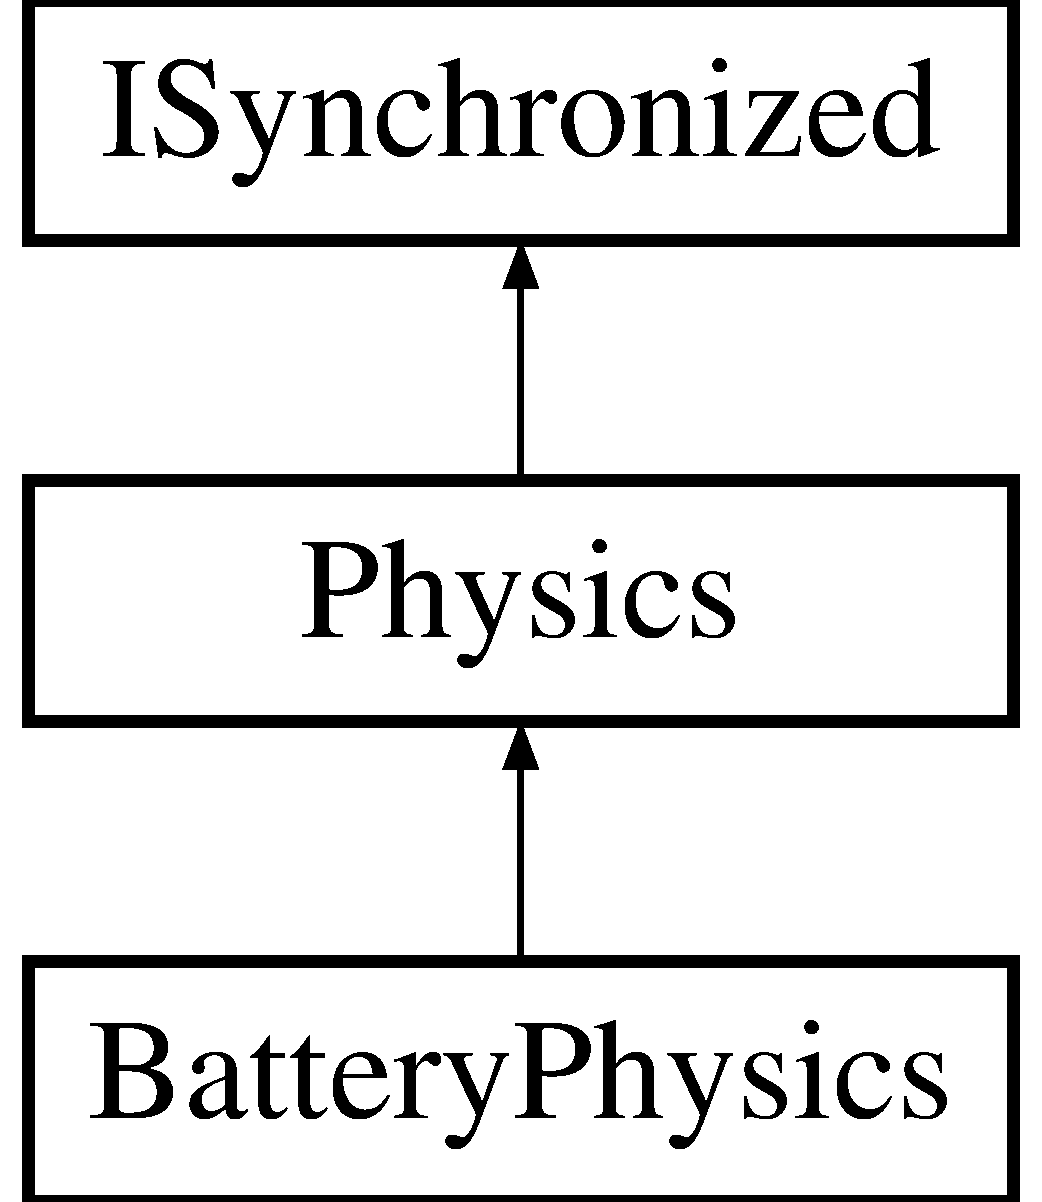
\includegraphics[height=3.000000cm]{classPhysics}
\end{center}
\end{figure}
\subsection*{Fonctions membres publiques}
\begin{DoxyCompactItemize}
\item 
\hypertarget{classPhysics_a6007da7545dc8ba917cd3b97439d4548}{{\bfseries Physics} (std\-::shared\-\_\-ptr$<$ \hyperlink{classModule}{Module} $>$)}\label{classPhysics_a6007da7545dc8ba917cd3b97439d4548}

\item 
\hypertarget{classPhysics_a041a4739fb28602797808c646c8018fa}{virtual void \hyperlink{classPhysics_a041a4739fb28602797808c646c8018fa}{clock} (int)=0}\label{classPhysics_a041a4739fb28602797808c646c8018fa}

\begin{DoxyCompactList}\small\item\em Méthode appellée à chaque pas de temps. \end{DoxyCompactList}\end{DoxyCompactItemize}
\subsection*{Attributs protégés}
\begin{DoxyCompactItemize}
\item 
\hypertarget{classPhysics_a059d7b72c91f5964fc3e3f3d5a189e9d}{std\-::shared\-\_\-ptr$<$ \hyperlink{classModule}{Module} $>$ {\bfseries module}}\label{classPhysics_a059d7b72c91f5964fc3e3f3d5a189e9d}

\end{DoxyCompactItemize}


\subsection{Description détaillée}
Classe abstraite pour décrire les différentes actions de l'environnement sur les modules. 

Prend en attribut un module dont elle à le droit de changer les paramètres. 

La documentation de cette classe a été générée à partir des fichiers suivants \-:\begin{DoxyCompactItemize}
\item 
src/\-Core/Physics.\-h\item 
src/\-Core/Physics.\-cpp\end{DoxyCompactItemize}

\hypertarget{classSocket}{\section{Référence de la classe Socket}
\label{classSocket}\index{Socket@{Socket}}
}


Classe abstraite pour les connecteurs des modules.  




{\ttfamily \#include $<$Socket.\-h$>$}

Graphe d'héritage de Socket\-:\begin{figure}[H]
\begin{center}
\leavevmode
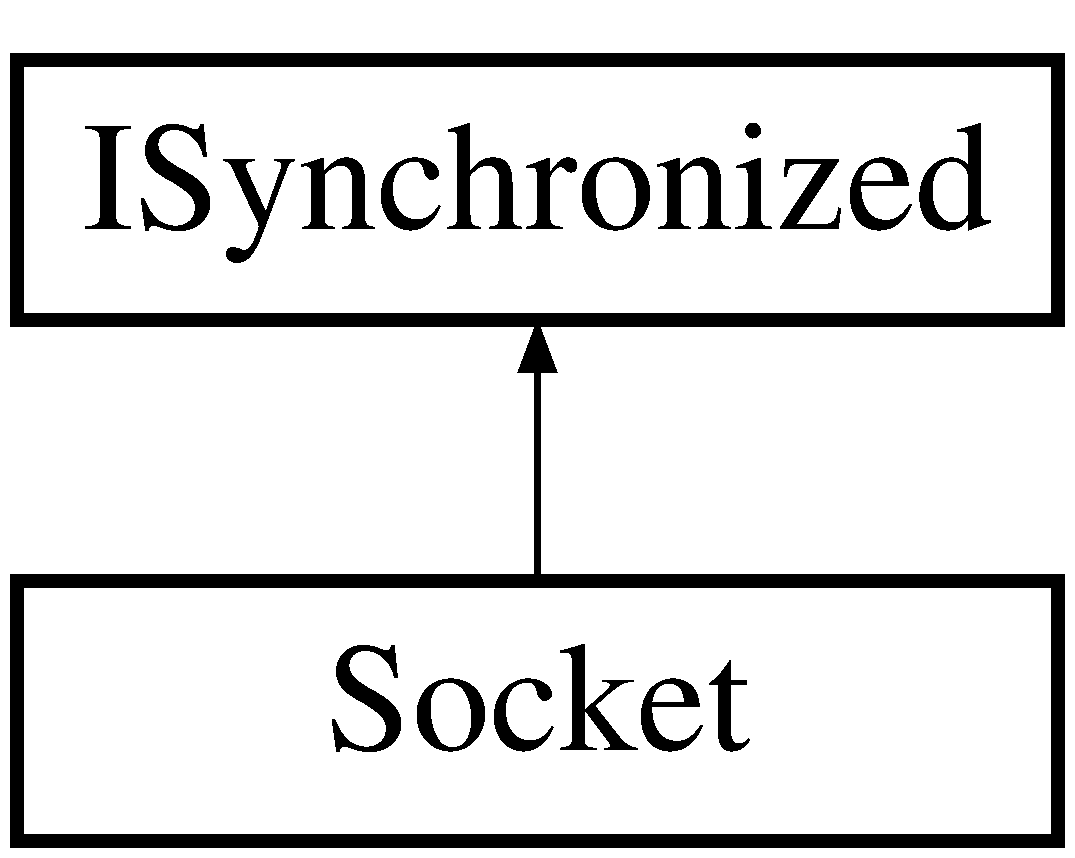
\includegraphics[height=2.000000cm]{classSocket}
\end{center}
\end{figure}
\subsection*{Fonctions membres publiques}
\begin{DoxyCompactItemize}
\item 
\hypertarget{classSocket_a0365662f7a20fa1cc6ef54fd2a659cfc}{{\bfseries Socket} (std\-::string name=\char`\"{}Socket\-Name\char`\"{}, std\-::string owner=\char`\"{}Socket\-Owner\char`\"{})}\label{classSocket_a0365662f7a20fa1cc6ef54fd2a659cfc}

\item 
\hypertarget{classSocket_a0dd97f1387c3bd8008cb7de47583a985}{{\bfseries Socket} (const \hyperlink{classSocket}{Socket} \&)}\label{classSocket_a0dd97f1387c3bd8008cb7de47583a985}

\item 
\hypertarget{classSocket_aeac4eb6379a543d38ed88977d3b6630a}{\hyperlink{classSocket_aeac4eb6379a543d38ed88977d3b6630a}{$\sim$\-Socket} ()}\label{classSocket_aeac4eb6379a543d38ed88977d3b6630a}

\begin{DoxyCompactList}\small\item\em Destructeur. \end{DoxyCompactList}\item 
\hypertarget{classSocket_a96d104e32d5f376796fb411874954e7d}{void \hyperlink{classSocket_a96d104e32d5f376796fb411874954e7d}{set\-Connexion} (\hyperlink{classConnexion}{Connexion} \&c)}\label{classSocket_a96d104e32d5f376796fb411874954e7d}

\begin{DoxyCompactList}\small\item\em Branche le socket à la connexion c. \end{DoxyCompactList}\item 
\hypertarget{classSocket_aaefa10006cbf7a7a082e4adc606b3cea}{std\-::string \hyperlink{classSocket_aaefa10006cbf7a7a082e4adc606b3cea}{get\-Name} ()}\label{classSocket_aaefa10006cbf7a7a082e4adc606b3cea}

\begin{DoxyCompactList}\small\item\em Retourne le nom de socket. \end{DoxyCompactList}\item 
\hypertarget{classSocket_a6421574ae64f7b40e7c3f7bbb5cc3cee}{std\-::string \hyperlink{classSocket_a6421574ae64f7b40e7c3f7bbb5cc3cee}{get\-Owner} ()}\label{classSocket_a6421574ae64f7b40e7c3f7bbb5cc3cee}

\begin{DoxyCompactList}\small\item\em Retourne le nom de module qui possede ce socket. \end{DoxyCompactList}\item 
\hypertarget{classSocket_a9adf799b90c455f3a1f4151adb031fd0}{void \hyperlink{classSocket_a9adf799b90c455f3a1f4151adb031fd0}{receive} (std\-::shared\-\_\-ptr$<$ \hyperlink{classMessage}{Message} $>$)}\label{classSocket_a9adf799b90c455f3a1f4151adb031fd0}

\begin{DoxyCompactList}\small\item\em Met le message m dans la file d'attente de socket. \end{DoxyCompactList}\item 
void \hyperlink{classSocket_a06b687baf9b01f3e399a5ee040ca04e4}{send} (std\-::shared\-\_\-ptr$<$ \hyperlink{classMessage}{Message} $>$)
\begin{DoxyCompactList}\small\item\em Envoye. \end{DoxyCompactList}\item 
\hypertarget{classSocket_a6bd5bddfabd838a3388b445c21d3c41e}{virtual void \hyperlink{classSocket_a6bd5bddfabd838a3388b445c21d3c41e}{clock} (int time)}\label{classSocket_a6bd5bddfabd838a3388b445c21d3c41e}

\begin{DoxyCompactList}\small\item\em Methode appellé à chaque tick d'horloge liée. \end{DoxyCompactList}\item 
\hypertarget{classSocket_afe7c9b2ef7fb3653b14f5f462293549a}{bool {\bfseries has\-Message} ()}\label{classSocket_afe7c9b2ef7fb3653b14f5f462293549a}

\item 
std\-::shared\-\_\-ptr$<$ \hyperlink{classMessage}{Message} $>$ \hyperlink{classSocket_a71e162a0ca00b1a46fe23eaccb09f76d}{get\-First\-Message} ()
\item 
\hypertarget{classSocket_aa890633022a29b56ed3844684d32e0fc}{int \hyperlink{classSocket_aa890633022a29b56ed3844684d32e0fc}{get\-Timer} () const }\label{classSocket_aa890633022a29b56ed3844684d32e0fc}

\begin{DoxyCompactList}\small\item\em Renvoie la valeur de timer. \end{DoxyCompactList}\end{DoxyCompactItemize}


\subsection{Description détaillée}
Classe abstraite pour les connecteurs des modules. 

\begin{DoxyRefDesc}{A faire}
\item[\hyperlink{todo__todo000011}{A faire}]Setconnection in \hyperlink{classSocket}{Socket} must be private and friend with Connection only ! \end{DoxyRefDesc}


Les sockets modélisent les connections entre les modules. Un connecteur peut-\/être soit un connecteur d'entrée, {\itshape In\-Socket}, soit un connecteur de sortie, {\itshape Out\-S\-Ocket}. Les connecteurs sont reliés entre-\/eux via les objets \hyperlink{classConnexion}{Connexion}. 

\subsection{Documentation des fonctions membres}
\hypertarget{classSocket_a71e162a0ca00b1a46fe23eaccb09f76d}{\index{Socket@{Socket}!get\-First\-Message@{get\-First\-Message}}
\index{get\-First\-Message@{get\-First\-Message}!Socket@{Socket}}
\subsubsection[{get\-First\-Message}]{\setlength{\rightskip}{0pt plus 5cm}std\-::shared\-\_\-ptr$<$ {\bf Message} $>$ Socket\-::get\-First\-Message (
\begin{DoxyParamCaption}
{}
\end{DoxyParamCaption}
)}}\label{classSocket_a71e162a0ca00b1a46fe23eaccb09f76d}
\begin{DoxyRefDesc}{A faire}
\item[\hyperlink{todo__todo000010}{A faire}]Lever une exception \end{DoxyRefDesc}
\hypertarget{classSocket_a06b687baf9b01f3e399a5ee040ca04e4}{\index{Socket@{Socket}!send@{send}}
\index{send@{send}!Socket@{Socket}}
\subsubsection[{send}]{\setlength{\rightskip}{0pt plus 5cm}void Socket\-::send (
\begin{DoxyParamCaption}
\item[{std\-::shared\-\_\-ptr$<$ {\bf Message} $>$}]{m}
\end{DoxyParamCaption}
)}}\label{classSocket_a06b687baf9b01f3e399a5ee040ca04e4}


Envoye. 

\begin{DoxyRefDesc}{A faire}
\item[\hyperlink{todo__todo000009}{A faire}]Et si connexion est null ? \end{DoxyRefDesc}


La documentation de cette classe a été générée à partir des fichiers suivants \-:\begin{DoxyCompactItemize}
\item 
src/\-Core/Socket.\-h\item 
src/\-Core/Socket.\-cpp\end{DoxyCompactItemize}

\hypertarget{classStringMessage}{\section{Référence de la classe String\-Message}
\label{classStringMessage}\index{String\-Message@{String\-Message}}
}


Classe de messages contenant une suite des caractères comme le payload.  




{\ttfamily \#include $<$String\-Message.\-h$>$}

Graphe d'héritage de String\-Message\-:\begin{figure}[H]
\begin{center}
\leavevmode
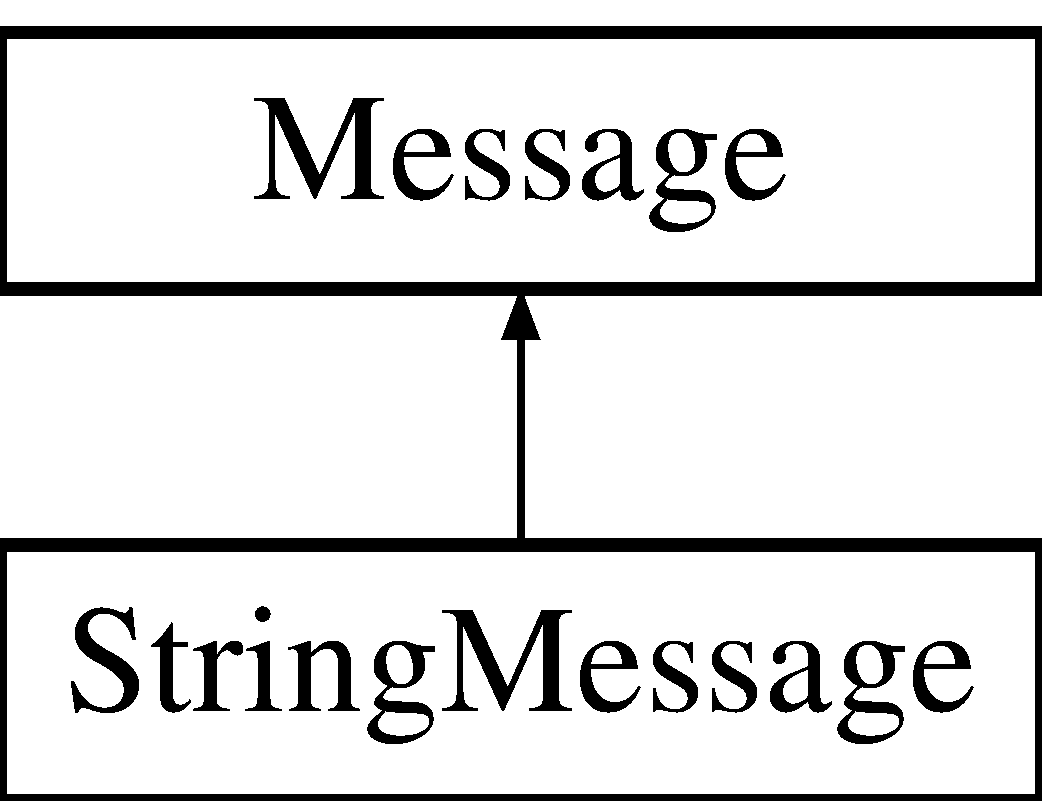
\includegraphics[height=2.000000cm]{classStringMessage}
\end{center}
\end{figure}
\subsection*{Fonctions membres publiques}
\begin{DoxyCompactItemize}
\item 
\hypertarget{classStringMessage_a205d7c1d64055e34ecd2f3f6664c7e6c}{{\bfseries String\-Message} (std\-::string \hyperlink{classMessage_ac7adddb666acdc47c48f684bd6810a51}{name}, std\-::string payload, int time=0)}\label{classStringMessage_a205d7c1d64055e34ecd2f3f6664c7e6c}

\item 
\hypertarget{classStringMessage_a5c8be5fb2d2d9e78be4e1fc303624610}{std\-::string \hyperlink{classStringMessage_a5c8be5fb2d2d9e78be4e1fc303624610}{get\-Payload} ()}\label{classStringMessage_a5c8be5fb2d2d9e78be4e1fc303624610}

\begin{DoxyCompactList}\small\item\em Renvoie la charge utile du message. \end{DoxyCompactList}\item 
\hypertarget{classStringMessage_a0071398acab934eb263ca6892ea76a4c}{std\-::ostream \& \hyperlink{classStringMessage_a0071398acab934eb263ca6892ea76a4c}{operator$<$$<$} (std\-::ostream \&os)}\label{classStringMessage_a0071398acab934eb263ca6892ea76a4c}

\begin{DoxyCompactList}\small\item\em Operateur de sortie surchargé \end{DoxyCompactList}\end{DoxyCompactItemize}
\subsection*{Membres hérités additionnels}


\subsection{Description détaillée}
Classe de messages contenant une suite des caractères comme le payload. 

La documentation de cette classe a été générée à partir des fichiers suivants \-:\begin{DoxyCompactItemize}
\item 
src/\-Core/\-Messages/String\-Message.\-h\item 
src/\-Core/\-Messages/String\-Message.\-cpp\end{DoxyCompactItemize}

\hypertarget{classTimer}{\section{Référence de la classe Timer}
\label{classTimer}\index{Timer@{Timer}}
}


Cette classe sert à la gestion du temps simulé  




{\ttfamily \#include $<$Timer.\-h$>$}

\subsection*{Fonctions membres publiques}
\begin{DoxyCompactItemize}
\item 
\hypertarget{classTimer_aeae0c417d77a86462b51da0615eab8b4}{void \hyperlink{classTimer_aeae0c417d77a86462b51da0615eab8b4}{add} (\hyperlink{classModule}{Module} $\ast$)}\label{classTimer_aeae0c417d77a86462b51da0615eab8b4}

\begin{DoxyCompactList}\small\item\em Ajouter le pointeur au module dans le tableau des modules synchronisés. \end{DoxyCompactList}\item 
\hypertarget{classTimer_a6cc5f746e08a0ec915123ef9687cb691}{void \hyperlink{classTimer_a6cc5f746e08a0ec915123ef9687cb691}{add} (\hyperlink{classPhysics}{Physics} $\ast$)}\label{classTimer_a6cc5f746e08a0ec915123ef9687cb691}

\begin{DoxyCompactList}\small\item\em Ajouter le pointeur au module dans le tableau des modules synchronisés. \end{DoxyCompactList}\item 
\hypertarget{classTimer_a62869fa83e1b76a9ebfe9cca7e56733d}{void \hyperlink{classTimer_a62869fa83e1b76a9ebfe9cca7e56733d}{start} (unsigned int c=100)}\label{classTimer_a62869fa83e1b76a9ebfe9cca7e56733d}

\begin{DoxyCompactList}\small\item\em Lancer le \hyperlink{classTimer}{Timer}. \end{DoxyCompactList}\item 
\hypertarget{classTimer_a63f0eb44b27402196590a03781515dba}{void \hyperlink{classTimer_a63f0eb44b27402196590a03781515dba}{stop} ()}\label{classTimer_a63f0eb44b27402196590a03781515dba}

\begin{DoxyCompactList}\small\item\em Arreter le \hyperlink{classTimer}{Timer}. \end{DoxyCompactList}\item 
\hypertarget{classTimer_a03ffd75bbb89ff1644839523af9fda03}{unsigned int \hyperlink{classTimer_a03ffd75bbb89ff1644839523af9fda03}{get\-Counter} () const }\label{classTimer_a03ffd75bbb89ff1644839523af9fda03}

\begin{DoxyCompactList}\small\item\em Retourne la valeur de compteur. \end{DoxyCompactList}\item 
\hypertarget{classTimer_a7394d4c4edb4d951dbe2c7e1ab2fb7ae}{void \hyperlink{classTimer_a7394d4c4edb4d951dbe2c7e1ab2fb7ae}{set\-Counter} (unsigned int)}\label{classTimer_a7394d4c4edb4d951dbe2c7e1ab2fb7ae}

\begin{DoxyCompactList}\small\item\em Mettre la valeur c dans le compteur. \end{DoxyCompactList}\end{DoxyCompactItemize}
\subsection*{Fonctions membres publiques statiques}
\begin{DoxyCompactItemize}
\item 
\hypertarget{classTimer_a8357f90f20707f9693fc713319de923a}{static \hyperlink{classTimer}{Timer} \& \hyperlink{classTimer_a8357f90f20707f9693fc713319de923a}{get\-Instance} ()}\label{classTimer_a8357f90f20707f9693fc713319de923a}

\begin{DoxyCompactList}\small\item\em Retourne l'instance unique de \hyperlink{classTimer}{Timer}. \end{DoxyCompactList}\end{DoxyCompactItemize}


\subsection{Description détaillée}
Cette classe sert à la gestion du temps simulé 

C'est le timer (unique) qui a pour rôle de synchroniser l'ensemble du simulateur et de donner les informations intéresantes sur le temps simulé. 

La documentation de cette classe a été générée à partir des fichiers suivants \-:\begin{DoxyCompactItemize}
\item 
src/\-Core/Timer.\-h\item 
src/\-Core/Timer.\-cpp\end{DoxyCompactItemize}

\hypertarget{classXMLReader}{\section{Référence de la classe X\-M\-L\-Reader}
\label{classXMLReader}\index{X\-M\-L\-Reader@{X\-M\-L\-Reader}}
}


Classe utilitaire pour la lecture des fichiers de configuration.  




{\ttfamily \#include $<$X\-M\-L\-Reader.\-h$>$}

\subsection*{Fonctions membres publiques}
\begin{DoxyCompactItemize}
\item 
\hypertarget{classXMLReader_a73065c7758f26ef69387e315c96d13ac}{\hyperlink{classXMLReader_a73065c7758f26ef69387e315c96d13ac}{$\sim$\-X\-M\-L\-Reader} ()}\label{classXMLReader_a73065c7758f26ef69387e315c96d13ac}

\begin{DoxyCompactList}\small\item\em Destructeur. \end{DoxyCompactList}\end{DoxyCompactItemize}
\subsection*{Fonctions membres publiques statiques}
\begin{DoxyCompactItemize}
\item 
static std\-::unordered\-\_\-map\\*
$<$ std\-::string, double $>$ \hyperlink{classXMLReader_a176f21253bd7ac73c00c0aa46e2e5724}{read\-Params} (std\-::string)
\begin{DoxyCompactList}\small\item\em Lecture des paramètre du module protant ce nom. Cette fonction recherche le fichier de configuration portant le nom du module, appelle le parser Rapid\-X\-M\-L puis créé le tableau de paramètres. En cas d'échec, elle lève une exception. \end{DoxyCompactList}\item 
\hypertarget{classXMLReader_aa21f5dcd9d009e635c6acad97beb240a}{static std\-::unordered\-\_\-map\\*
$<$ std\-::string, int $>$ \hyperlink{classXMLReader_aa21f5dcd9d009e635c6acad97beb240a}{read\-Messages} (std\-::string)}\label{classXMLReader_aa21f5dcd9d009e635c6acad97beb240a}

\begin{DoxyCompactList}\small\item\em Lecture des méssages compris par le module protant ce nom. Cette fonction recherche le fichier de configuration portant le nom du module, appelle le parser Rapid\-X\-M\-L puis créé le tableau de messages. En cas d'échec, elle lève une exception. \end{DoxyCompactList}\item 
\hypertarget{classXMLReader_af23225be3e3a4db017f1e22d1b21f7eb}{static std\-::vector$<$ std\-::string $>$ \hyperlink{classXMLReader_af23225be3e3a4db017f1e22d1b21f7eb}{read\-Sockets} (std\-::string)}\label{classXMLReader_af23225be3e3a4db017f1e22d1b21f7eb}

\begin{DoxyCompactList}\small\item\em Lecture des sockets de modile portant ce nom. Cette fonction recherche le fichier de configuration portant le nom du module, appelle le parser Rapid\-X\-M\-L puis créé le tableau de noms de sockets. En cas d'échec, elle lève une exception. \end{DoxyCompactList}\item 
\hypertarget{classXMLReader_a5147abbb0cacd3fbcc396a23cc63456b}{static std\-::string \hyperlink{classXMLReader_a5147abbb0cacd3fbcc396a23cc63456b}{get\-Path} ()}\label{classXMLReader_a5147abbb0cacd3fbcc396a23cc63456b}

\begin{DoxyCompactList}\small\item\em Getter statique du chemin vers le dossier de configuration. \end{DoxyCompactList}\item 
\hypertarget{classXMLReader_ae8d2d4fd99c45bc46b939d9dc3548340}{static void \hyperlink{classXMLReader_ae8d2d4fd99c45bc46b939d9dc3548340}{set\-Path} (std\-::string)}\label{classXMLReader_ae8d2d4fd99c45bc46b939d9dc3548340}

\begin{DoxyCompactList}\small\item\em Setter statique du chemin vers le dossier de configuration. \end{DoxyCompactList}\end{DoxyCompactItemize}


\subsection{Description détaillée}
Classe utilitaire pour la lecture des fichiers de configuration. 

Cette classe statique fournit des méthodes statiques permettant par exemple de lire la configuration initiale du simulateur dans les fihciers xml 

\subsection{Documentation des fonctions membres}
\hypertarget{classXMLReader_a176f21253bd7ac73c00c0aa46e2e5724}{\index{X\-M\-L\-Reader@{X\-M\-L\-Reader}!read\-Params@{read\-Params}}
\index{read\-Params@{read\-Params}!XMLReader@{X\-M\-L\-Reader}}
\subsubsection[{read\-Params}]{\setlength{\rightskip}{0pt plus 5cm}static std\-::unordered\-\_\-map$<$ std\-::string, double $>$ X\-M\-L\-Reader\-::read\-Params (
\begin{DoxyParamCaption}
\item[{std\-::string}]{module\-Name}
\end{DoxyParamCaption}
)\hspace{0.3cm}{\ttfamily [static]}}}\label{classXMLReader_a176f21253bd7ac73c00c0aa46e2e5724}


Lecture des paramètre du module protant ce nom. Cette fonction recherche le fichier de configuration portant le nom du module, appelle le parser Rapid\-X\-M\-L puis créé le tableau de paramètres. En cas d'échec, elle lève une exception. 

Le chemin vers le dossier de configuration 

La documentation de cette classe a été générée à partir des fichiers suivants \-:\begin{DoxyCompactItemize}
\item 
src/\-Core/X\-M\-L\-Reader.\-h\item 
src/\-Core/X\-M\-L\-Reader.\-cpp\end{DoxyCompactItemize}

\printindex
\end{document}
